\documentclass[english]{article}
\usepackage[utf8]{inputenc}
\usepackage[T1]{fontenc}
\usepackage{babel}
\usepackage{svg}
\usepackage{caption, booktabs}
\usepackage{amsmath}
\usepackage{graphicx}
\usepackage{fancyhdr}
\usepackage{todonotes}
\usepackage{units}
\usepackage[
	colorlinks=true,
	urlcolor=blue,
	linkcolor=green
]{hyperref}
\newcommand{\scidatalogo}{
\includegraphics[height=36pt]{SciData_logo.jpg}}
\pagestyle{fancy}
\fancyhf{}
\renewcommand{\headrulewidth}{0pt}
\setlength{\headheight}{40pt}
\lhead{\textsc{\scidatalogo}}
\usepackage{natbib}

\begin{document}
\newcommand{\aoBodyAll}{66}
\newcommand{\aoBodyI}{6}
\newcommand{\aoBodyII}{12}
\newcommand{\aoBodyIII}{7}
\newcommand{\aoBodyIV}{12}
\newcommand{\aoBodyV}{2}
\newcommand{\aoBodyVI}{9}
\newcommand{\aoBodyVII}{13}
\newcommand{\aoBodyVIII}{5}

\newcommand{\aoBpartAll}{69}
\newcommand{\aoBpartI}{9}
\newcommand{\aoBpartII}{8}
\newcommand{\aoBpartIII}{6}
\newcommand{\aoBpartIV}{13}
\newcommand{\aoBpartV}{5}
\newcommand{\aoBpartVI}{7}
\newcommand{\aoBpartVII}{11}
\newcommand{\aoBpartVIII}{10}

\newcommand{\aoFaheadAll}{83}
\newcommand{\aoFaheadI}{12}
\newcommand{\aoFaheadII}{11}
\newcommand{\aoFaheadIII}{10}
\newcommand{\aoFaheadIV}{5}
\newcommand{\aoFaheadV}{9}
\newcommand{\aoFaheadVI}{13}
\newcommand{\aoFaheadVII}{12}
\newcommand{\aoFaheadVIII}{11}

\newcommand{\aoFgadlrdiffAll}{180133}
\newcommand{\aoFgadlrdiffI}{22574}
\newcommand{\aoFgadlrdiffII}{22075}
\newcommand{\aoFgadlrdiffIII}{21925}
\newcommand{\aoFgadlrdiffIV}{24425}
\newcommand{\aoFgadlrdiffV}{23125}
\newcommand{\aoFgadlrdiffVI}{21975}
\newcommand{\aoFgadlrdiffVII}{27175}
\newcommand{\aoFgadlrdiffVIII}{16859}

\newcommand{\aoFgadrmsAll}{180133}
\newcommand{\aoFgadrmsI}{22574}
\newcommand{\aoFgadrmsII}{22075}
\newcommand{\aoFgadrmsIII}{21925}
\newcommand{\aoFgadrmsIV}{24425}
\newcommand{\aoFgadrmsV}{23125}
\newcommand{\aoFgadrmsVI}{21975}
\newcommand{\aoFgadrmsVII}{27175}
\newcommand{\aoFgadrmsVIII}{16859}

\newcommand{\aoFurnAll}{50}
\newcommand{\aoFurnI}{8}
\newcommand{\aoFurnII}{5}
\newcommand{\aoFurnIII}{2}
\newcommand{\aoFurnIV}{5}
\newcommand{\aoFurnV}{7}
\newcommand{\aoFurnVI}{10}
\newcommand{\aoFurnVII}{7}
\newcommand{\aoFurnVIII}{6}

\newcommand{\aoGeoAll}{125}
\newcommand{\aoGeoI}{16}
\newcommand{\aoGeoII}{17}
\newcommand{\aoGeoIII}{11}
\newcommand{\aoGeoIV}{32}
\newcommand{\aoGeoV}{0}
\newcommand{\aoGeoVI}{15}
\newcommand{\aoGeoVII}{18}
\newcommand{\aoGeoVIII}{16}

\newcommand{\aoGroomAll}{105}
\newcommand{\aoGroomI}{12}
\newcommand{\aoGroomII}{11}
\newcommand{\aoGroomIII}{8}
\newcommand{\aoGroomIV}{5}
\newcommand{\aoGroomV}{8}
\newcommand{\aoGroomVI}{25}
\newcommand{\aoGroomVII}{28}
\newcommand{\aoGroomVIII}{8}

\newcommand{\aoObjAll}{284}
\newcommand{\aoObjI}{39}
\newcommand{\aoObjII}{34}
\newcommand{\aoObjIII}{27}
\newcommand{\aoObjIV}{44}
\newcommand{\aoObjV}{29}
\newcommand{\aoObjVI}{42}
\newcommand{\aoObjVII}{32}
\newcommand{\aoObjVIII}{37}

\newcommand{\aoSenewAll}{86}
\newcommand{\aoSenewI}{11}
\newcommand{\aoSenewII}{15}
\newcommand{\aoSenewIII}{12}
\newcommand{\aoSenewIV}{4}
\newcommand{\aoSenewV}{15}
\newcommand{\aoSenewVI}{10}
\newcommand{\aoSenewVII}{16}
\newcommand{\aoSenewVIII}{3}

\newcommand{\aoSeoldAll}{37}
\newcommand{\aoSeoldI}{2}
\newcommand{\aoSeoldII}{5}
\newcommand{\aoSeoldIII}{1}
\newcommand{\aoSeoldIV}{4}
\newcommand{\aoSeoldV}{2}
\newcommand{\aoSeoldVI}{9}
\newcommand{\aoSeoldVII}{8}
\newcommand{\aoSeoldVIII}{6}

\newcommand{\aoSexfAll}{108}
\newcommand{\aoSexfI}{14}
\newcommand{\aoSexfII}{22}
\newcommand{\aoSexfIII}{6}
\newcommand{\aoSexfIV}{6}
\newcommand{\aoSexfV}{13}
\newcommand{\aoSexfVI}{10}
\newcommand{\aoSexfVII}{23}
\newcommand{\aoSexfVIII}{14}

\newcommand{\aoSexmAll}{403}
\newcommand{\aoSexmI}{41}
\newcommand{\aoSexmII}{68}
\newcommand{\aoSexmIII}{38}
\newcommand{\aoSexmIV}{102}
\newcommand{\aoSexmV}{45}
\newcommand{\aoSexmVI}{42}
\newcommand{\aoSexmVII}{42}
\newcommand{\aoSexmVIII}{25}

\newcommand{\aoSexuAll}{17}
\newcommand{\aoSexuI}{0}
\newcommand{\aoSexuII}{3}
\newcommand{\aoSexuIII}{1}
\newcommand{\aoSexuIV}{2}
\newcommand{\aoSexuV}{3}
\newcommand{\aoSexuVI}{1}
\newcommand{\aoSexuVII}{5}
\newcommand{\aoSexuVIII}{2}

\newcommand{\aoVlochAll}{89}
\newcommand{\aoVlochI}{10}
\newcommand{\aoVlochII}{31}
\newcommand{\aoVlochIII}{2}
\newcommand{\aoVlochIV}{23}
\newcommand{\aoVlochV}{4}
\newcommand{\aoVlochVI}{18}
\newcommand{\aoVlochVII}{1}
\newcommand{\aoVnocutAll}{148}
\newcommand{\aoVnocutI}{30}
\newcommand{\aoVnocutII}{13}
\newcommand{\aoVnocutIII}{21}
\newcommand{\aoVnocutIV}{15}
\newcommand{\aoVnocutV}{27}
\newcommand{\aoVnocutVI}{9}
\newcommand{\aoVnocutVII}{17}
\newcommand{\aoVnocutVIII}{16}

\newcommand{\aoVpenewAll}{386}
\newcommand{\aoVpenewI}{31}
\newcommand{\aoVpenewII}{38}
\newcommand{\aoVpenewIII}{72}
\newcommand{\aoVpenewIV}{90}
\newcommand{\aoVpenewV}{89}
\newcommand{\aoVpenewVI}{33}
\newcommand{\aoVpenewVII}{24}
\newcommand{\aoVpenewVIII}{9}

\newcommand{\aoVpeoldAll}{208}
\newcommand{\aoVpeoldI}{25}
\newcommand{\aoVpeoldII}{61}
\newcommand{\aoVpeoldIII}{13}
\newcommand{\aoVpeoldIV}{1}
\newcommand{\aoVpeoldV}{32}
\newcommand{\aoVpeoldVI}{29}
\newcommand{\aoVpeoldVII}{47}
\newcommand{\aoVsenewAll}{96}
\newcommand{\aoVsenewI}{11}
\newcommand{\aoVsenewII}{14}
\newcommand{\aoVsenewIII}{17}
\newcommand{\aoVsenewIV}{4}
\newcommand{\aoVsenewV}{17}
\newcommand{\aoVsenewVI}{9}
\newcommand{\aoVsenewVII}{21}
\newcommand{\aoVsenewVIII}{3}

\newcommand{\aoVseoldAll}{90}
\newcommand{\aoVseoldI}{7}
\newcommand{\aoVseoldII}{11}
\newcommand{\aoVseoldIII}{3}
\newcommand{\aoVseoldIV}{7}
\newcommand{\aoVseoldV}{7}
\newcommand{\aoVseoldVI}{23}
\newcommand{\aoVseoldVII}{15}
\newcommand{\aoVseoldVIII}{17}


\newcommand{\avBodyAll}{66}
\newcommand{\avBodyI}{6}
\newcommand{\avBodyII}{12}
\newcommand{\avBodyIII}{7}
\newcommand{\avBodyIV}{12}
\newcommand{\avBodyV}{2}
\newcommand{\avBodyVI}{9}
\newcommand{\avBodyVII}{13}
\newcommand{\avBodyVIII}{5}

\newcommand{\avBpartAll}{69}
\newcommand{\avBpartI}{9}
\newcommand{\avBpartII}{8}
\newcommand{\avBpartIII}{6}
\newcommand{\avBpartIV}{13}
\newcommand{\avBpartV}{5}
\newcommand{\avBpartVI}{7}
\newcommand{\avBpartVII}{11}
\newcommand{\avBpartVIII}{10}

\newcommand{\avFaheadAll}{83}
\newcommand{\avFaheadI}{12}
\newcommand{\avFaheadII}{11}
\newcommand{\avFaheadIII}{10}
\newcommand{\avFaheadIV}{5}
\newcommand{\avFaheadV}{9}
\newcommand{\avFaheadVI}{13}
\newcommand{\avFaheadVII}{12}
\newcommand{\avFaheadVIII}{11}

\newcommand{\avFgavgerlrAll}{180783}
\newcommand{\avFgavgerlrI}{22656}
\newcommand{\avFgavgerlrII}{22158}
\newcommand{\avFgavgerlrIII}{22008}
\newcommand{\avFgavgerlrIV}{24507}
\newcommand{\avFgavgerlrV}{23208}
\newcommand{\avFgavgerlrVI}{22057}
\newcommand{\avFgavgerlrVII}{27208}
\newcommand{\avFgavgerlrVIII}{16981}

\newcommand{\avFgavgerlrdiffAll}{180759}
\newcommand{\avFgavgerlrdiffI}{22653}
\newcommand{\avFgavgerlrdiffII}{22155}
\newcommand{\avFgavgerlrdiffIII}{22005}
\newcommand{\avFgavgerlrdiffIV}{24504}
\newcommand{\avFgavgerlrdiffV}{23205}
\newcommand{\avFgavgerlrdiffVI}{22054}
\newcommand{\avFgavgerlrdiffVII}{27205}
\newcommand{\avFgavgerlrdiffVIII}{16978}

\newcommand{\avFgavgermlAll}{180783}
\newcommand{\avFgavgermlI}{22656}
\newcommand{\avFgavgermlII}{22158}
\newcommand{\avFgavgermlIII}{22008}
\newcommand{\avFgavgermlIV}{24507}
\newcommand{\avFgavgermlV}{23208}
\newcommand{\avFgavgermlVI}{22057}
\newcommand{\avFgavgermlVII}{27208}
\newcommand{\avFgavgermlVIII}{16981}

\newcommand{\avFgavgerpdAll}{180783}
\newcommand{\avFgavgerpdI}{22656}
\newcommand{\avFgavgerpdII}{22158}
\newcommand{\avFgavgerpdIII}{22008}
\newcommand{\avFgavgerpdIV}{24507}
\newcommand{\avFgavgerpdV}{23208}
\newcommand{\avFgavgerpdVI}{22057}
\newcommand{\avFgavgerpdVII}{27208}
\newcommand{\avFgavgerpdVIII}{16981}

\newcommand{\avFgavgerrmsAll}{180759}
\newcommand{\avFgavgerrmsI}{22653}
\newcommand{\avFgavgerrmsII}{22155}
\newcommand{\avFgavgerrmsIII}{22005}
\newcommand{\avFgavgerrmsIV}{24504}
\newcommand{\avFgavgerrmsV}{23205}
\newcommand{\avFgavgerrmsVI}{22054}
\newcommand{\avFgavgerrmsVII}{27205}
\newcommand{\avFgavgerrmsVIII}{16978}

\newcommand{\avFgavgerudAll}{180783}
\newcommand{\avFgavgerudI}{22656}
\newcommand{\avFgavgerudII}{22158}
\newcommand{\avFgavgerudIII}{22008}
\newcommand{\avFgavgerudIV}{24507}
\newcommand{\avFgavgerudV}{23208}
\newcommand{\avFgavgerudVI}{22057}
\newcommand{\avFgavgerudVII}{27208}
\newcommand{\avFgavgerudVIII}{16981}

\newcommand{\avFurnAll}{50}
\newcommand{\avFurnI}{8}
\newcommand{\avFurnII}{5}
\newcommand{\avFurnIII}{2}
\newcommand{\avFurnIV}{5}
\newcommand{\avFurnV}{7}
\newcommand{\avFurnVI}{10}
\newcommand{\avFurnVII}{7}
\newcommand{\avFurnVIII}{6}

\newcommand{\avGeoAll}{125}
\newcommand{\avGeoI}{16}
\newcommand{\avGeoII}{17}
\newcommand{\avGeoIII}{11}
\newcommand{\avGeoIV}{32}
\newcommand{\avGeoV}{0}
\newcommand{\avGeoVI}{15}
\newcommand{\avGeoVII}{18}
\newcommand{\avGeoVIII}{16}

\newcommand{\avGroomAll}{105}
\newcommand{\avGroomI}{12}
\newcommand{\avGroomII}{11}
\newcommand{\avGroomIII}{8}
\newcommand{\avGroomIV}{5}
\newcommand{\avGroomV}{8}
\newcommand{\avGroomVI}{25}
\newcommand{\avGroomVII}{28}
\newcommand{\avGroomVIII}{8}

\newcommand{\avObjAll}{284}
\newcommand{\avObjI}{39}
\newcommand{\avObjII}{34}
\newcommand{\avObjIII}{27}
\newcommand{\avObjIV}{44}
\newcommand{\avObjV}{29}
\newcommand{\avObjVI}{42}
\newcommand{\avObjVII}{32}
\newcommand{\avObjVIII}{37}

\newcommand{\avSenewAll}{86}
\newcommand{\avSenewI}{11}
\newcommand{\avSenewII}{15}
\newcommand{\avSenewIII}{12}
\newcommand{\avSenewIV}{4}
\newcommand{\avSenewV}{15}
\newcommand{\avSenewVI}{10}
\newcommand{\avSenewVII}{16}
\newcommand{\avSenewVIII}{3}

\newcommand{\avSeoldAll}{37}
\newcommand{\avSeoldI}{2}
\newcommand{\avSeoldII}{5}
\newcommand{\avSeoldIII}{1}
\newcommand{\avSeoldIV}{4}
\newcommand{\avSeoldV}{2}
\newcommand{\avSeoldVI}{9}
\newcommand{\avSeoldVII}{8}
\newcommand{\avSeoldVIII}{6}

\newcommand{\avSexfAll}{108}
\newcommand{\avSexfI}{14}
\newcommand{\avSexfII}{22}
\newcommand{\avSexfIII}{6}
\newcommand{\avSexfIV}{6}
\newcommand{\avSexfV}{13}
\newcommand{\avSexfVI}{10}
\newcommand{\avSexfVII}{23}
\newcommand{\avSexfVIII}{14}

\newcommand{\avSexmAll}{403}
\newcommand{\avSexmI}{41}
\newcommand{\avSexmII}{68}
\newcommand{\avSexmIII}{38}
\newcommand{\avSexmIV}{102}
\newcommand{\avSexmV}{45}
\newcommand{\avSexmVI}{42}
\newcommand{\avSexmVII}{42}
\newcommand{\avSexmVIII}{25}

\newcommand{\avSexuAll}{17}
\newcommand{\avSexuI}{0}
\newcommand{\avSexuII}{3}
\newcommand{\avSexuIII}{1}
\newcommand{\avSexuIV}{2}
\newcommand{\avSexuV}{3}
\newcommand{\avSexuVI}{1}
\newcommand{\avSexuVII}{5}
\newcommand{\avSexuVIII}{2}

\newcommand{\avVlochAll}{89}
\newcommand{\avVlochI}{10}
\newcommand{\avVlochII}{31}
\newcommand{\avVlochIII}{2}
\newcommand{\avVlochIV}{23}
\newcommand{\avVlochV}{4}
\newcommand{\avVlochVI}{18}
\newcommand{\avVlochVII}{1}
\newcommand{\avVnocutAll}{148}
\newcommand{\avVnocutI}{30}
\newcommand{\avVnocutII}{13}
\newcommand{\avVnocutIII}{21}
\newcommand{\avVnocutIV}{15}
\newcommand{\avVnocutV}{27}
\newcommand{\avVnocutVI}{9}
\newcommand{\avVnocutVII}{17}
\newcommand{\avVnocutVIII}{16}

\newcommand{\avVpenewAll}{386}
\newcommand{\avVpenewI}{31}
\newcommand{\avVpenewII}{38}
\newcommand{\avVpenewIII}{72}
\newcommand{\avVpenewIV}{90}
\newcommand{\avVpenewV}{89}
\newcommand{\avVpenewVI}{33}
\newcommand{\avVpenewVII}{24}
\newcommand{\avVpenewVIII}{9}

\newcommand{\avVpeoldAll}{208}
\newcommand{\avVpeoldI}{25}
\newcommand{\avVpeoldII}{61}
\newcommand{\avVpeoldIII}{13}
\newcommand{\avVpeoldIV}{1}
\newcommand{\avVpeoldV}{32}
\newcommand{\avVpeoldVI}{29}
\newcommand{\avVpeoldVII}{47}
\newcommand{\avVsenewAll}{96}
\newcommand{\avVsenewI}{11}
\newcommand{\avVsenewII}{14}
\newcommand{\avVsenewIII}{17}
\newcommand{\avVsenewIV}{4}
\newcommand{\avVsenewV}{17}
\newcommand{\avVsenewVI}{9}
\newcommand{\avVsenewVII}{21}
\newcommand{\avVsenewVIII}{3}

\newcommand{\avVseoldAll}{90}
\newcommand{\avVseoldI}{7}
\newcommand{\avVseoldII}{11}
\newcommand{\avVseoldIII}{3}
\newcommand{\avVseoldIV}{7}
\newcommand{\avVseoldV}{7}
\newcommand{\avVseoldVI}{23}
\newcommand{\avVseoldVII}{15}
\newcommand{\avVseoldVIII}{17}


\newcommand{\anAll}{17}
\newcommand{\anI}{2}
\newcommand{\anII}{2}
\newcommand{\anIII}{2}
\newcommand{\anIV}{0}
\newcommand{\anV}{3}
\newcommand{\anVI}{3}
\newcommand{\anVII}{4}
\newcommand{\anVIII}{1}

\newcommand{\anBodyAll}{66}
\newcommand{\anBodyI}{6}
\newcommand{\anBodyII}{12}
\newcommand{\anBodyIII}{7}
\newcommand{\anBodyIV}{12}
\newcommand{\anBodyV}{2}
\newcommand{\anBodyVI}{9}
\newcommand{\anBodyVII}{13}
\newcommand{\anBodyVIII}{5}

\newcommand{\anBodypartAll}{69}
\newcommand{\anBodypartI}{9}
\newcommand{\anBodypartII}{8}
\newcommand{\anBodypartIII}{6}
\newcommand{\anBodypartIV}{13}
\newcommand{\anBodypartV}{5}
\newcommand{\anBodypartVI}{7}
\newcommand{\anBodypartVII}{11}
\newcommand{\anBodypartVIII}{10}

\newcommand{\anFaceAll}{47}
\newcommand{\anFaceI}{7}
\newcommand{\anFaceII}{7}
\newcommand{\anFaceIII}{6}
\newcommand{\anFaceIV}{1}
\newcommand{\anFaceV}{7}
\newcommand{\anFaceVI}{9}
\newcommand{\anFaceVII}{6}
\newcommand{\anFaceVIII}{4}

\newcommand{\anFemaleAll}{31}
\newcommand{\anFemaleI}{12}
\newcommand{\anFemaleII}{8}
\newcommand{\anFemaleIII}{0}
\newcommand{\anFemaleIV}{3}
\newcommand{\anFemaleV}{0}
\newcommand{\anFemaleVI}{3}
\newcommand{\anFemaleVII}{2}
\newcommand{\anFemaleVIII}{3}

\newcommand{\anFemalesAll}{3}
\newcommand{\anFemalesI}{0}
\newcommand{\anFemalesII}{0}
\newcommand{\anFemalesIII}{0}
\newcommand{\anFemalesIV}{2}
\newcommand{\anFemalesV}{0}
\newcommand{\anFemalesVI}{0}
\newcommand{\anFemalesVII}{1}
\newcommand{\anFemalesVIII}{0}

\newcommand{\anFnameAll}{74}
\newcommand{\anFnameI}{2}
\newcommand{\anFnameII}{14}
\newcommand{\anFnameIII}{6}
\newcommand{\anFnameIV}{1}
\newcommand{\anFnameV}{13}
\newcommand{\anFnameVI}{7}
\newcommand{\anFnameVII}{20}
\newcommand{\anFnameVIII}{11}

\newcommand{\anFurnitureAll}{50}
\newcommand{\anFurnitureI}{8}
\newcommand{\anFurnitureII}{5}
\newcommand{\anFurnitureIII}{2}
\newcommand{\anFurnitureIV}{5}
\newcommand{\anFurnitureV}{7}
\newcommand{\anFurnitureVI}{10}
\newcommand{\anFurnitureVII}{7}
\newcommand{\anFurnitureVIII}{6}

\newcommand{\anGeoAll}{125}
\newcommand{\anGeoI}{16}
\newcommand{\anGeoII}{17}
\newcommand{\anGeoIII}{11}
\newcommand{\anGeoIV}{32}
\newcommand{\anGeoV}{0}
\newcommand{\anGeoVI}{15}
\newcommand{\anGeoVII}{18}
\newcommand{\anGeoVIII}{16}

\newcommand{\anGeoroomAll}{105}
\newcommand{\anGeoroomI}{12}
\newcommand{\anGeoroomII}{11}
\newcommand{\anGeoroomIII}{8}
\newcommand{\anGeoroomIV}{5}
\newcommand{\anGeoroomV}{8}
\newcommand{\anGeoroomVI}{25}
\newcommand{\anGeoroomVII}{28}
\newcommand{\anGeoroomVIII}{8}

\newcommand{\anHeadAll}{36}
\newcommand{\anHeadI}{5}
\newcommand{\anHeadII}{4}
\newcommand{\anHeadIII}{4}
\newcommand{\anHeadIV}{4}
\newcommand{\anHeadV}{2}
\newcommand{\anHeadVI}{4}
\newcommand{\anHeadVII}{6}
\newcommand{\anHeadVIII}{7}

\newcommand{\anMaleAll}{89}
\newcommand{\anMaleI}{15}
\newcommand{\anMaleII}{18}
\newcommand{\anMaleIII}{9}
\newcommand{\anMaleIV}{18}
\newcommand{\anMaleV}{7}
\newcommand{\anMaleVI}{8}
\newcommand{\anMaleVII}{9}
\newcommand{\anMaleVIII}{5}

\newcommand{\anMalesAll}{23}
\newcommand{\anMalesI}{2}
\newcommand{\anMalesII}{11}
\newcommand{\anMalesIII}{4}
\newcommand{\anMalesIV}{3}
\newcommand{\anMalesV}{2}
\newcommand{\anMalesVI}{0}
\newcommand{\anMalesVII}{1}
\newcommand{\anMalesVIII}{0}

\newcommand{\anMnameAll}{291}
\newcommand{\anMnameI}{24}
\newcommand{\anMnameII}{39}
\newcommand{\anMnameIII}{25}
\newcommand{\anMnameIV}{81}
\newcommand{\anMnameV}{36}
\newcommand{\anMnameVI}{34}
\newcommand{\anMnameVII}{32}
\newcommand{\anMnameVIII}{20}

\newcommand{\anObjectAll}{232}
\newcommand{\anObjectI}{36}
\newcommand{\anObjectII}{22}
\newcommand{\anObjectIII}{20}
\newcommand{\anObjectIV}{30}
\newcommand{\anObjectV}{25}
\newcommand{\anObjectVI}{37}
\newcommand{\anObjectVII}{26}
\newcommand{\anObjectVIII}{36}

\newcommand{\anObjectsAll}{52}
\newcommand{\anObjectsI}{3}
\newcommand{\anObjectsII}{12}
\newcommand{\anObjectsIII}{7}
\newcommand{\anObjectsIV}{14}
\newcommand{\anObjectsV}{4}
\newcommand{\anObjectsVI}{5}
\newcommand{\anObjectsVII}{6}
\newcommand{\anObjectsVIII}{1}

\newcommand{\anPersonsAll}{17}
\newcommand{\anPersonsI}{0}
\newcommand{\anPersonsII}{3}
\newcommand{\anPersonsIII}{1}
\newcommand{\anPersonsIV}{2}
\newcommand{\anPersonsV}{3}
\newcommand{\anPersonsVI}{1}
\newcommand{\anPersonsVII}{5}
\newcommand{\anPersonsVIII}{2}

\newcommand{\anSettingnewAll}{86}
\newcommand{\anSettingnewI}{11}
\newcommand{\anSettingnewII}{15}
\newcommand{\anSettingnewIII}{12}
\newcommand{\anSettingnewIV}{4}
\newcommand{\anSettingnewV}{15}
\newcommand{\anSettingnewVI}{10}
\newcommand{\anSettingnewVII}{16}
\newcommand{\anSettingnewVIII}{3}

\newcommand{\anSettingrecAll}{37}
\newcommand{\anSettingrecI}{2}
\newcommand{\anSettingrecII}{5}
\newcommand{\anSettingrecIII}{1}
\newcommand{\anSettingrecIV}{4}
\newcommand{\anSettingrecV}{2}
\newcommand{\anSettingrecVI}{9}
\newcommand{\anSettingrecVII}{8}
\newcommand{\anSettingrecVIII}{6}



% title has to be < 110 chars incl. spaces
%  at the moment 109 Chars
\title{Hemodynamic responses of the Parahippocampal Place Area to spatial cues in a movie and its audio-description}

\author{Christian~O.~Häusler\textsuperscript{1,2{*}}, Michael
Hanke\textsuperscript{1,2}}
% https://www.nature.com/sdata/publish/for-authors#other-formats

\maketitle
\thispagestyle{fancy}

1. Psychoinformatics Lab, Institute of Neuroscience and Medicine, Brain \&
Behaviour (INM-7), Research Centre Jülich, Jülich, Germany, 2. Institute of
Systems Neuroscience, Medical Faculty, Heinrich Heine University,  Düsseldorf,
Germany {*}corresponding author: Christian Olaf Häusler (der.haeusler@gmx.net)

\begin{abstract}
% < 170 words new analysis of existing data of interest to a broad section of
% our audience highlighting innovative examples of data reuse may be used to
% present compelling new findings & conclusions derived from published.
Intro: PPA as classic example for an visual area; Methods: fMRI data
studyforrest data set, general linear model; Results: significant clusters in
PPA, RSC, individual results in x of 15 subjects; Conclusions: results suggest
generalizability to spoken language and is restricted to processing visual
stimuli exclusively. \end{abstract}


\todo[inline]{our system cannot accept BibTeX bibliography files; authors who
    wish to use BibTeX to prepare their references should therefore copy the
    reference list from the .bbl file that BibTeX generates and paste it into
    the main manuscript .tex file (and delete the associated
    \textbackslash{}bibliography and \textbackslash{}bibliographystyle
commands)}


\section{Introduction}
\todo[inline]{I wonder whether we should make a general point: The construction
  of contrasts of interests feels "messy". But this is a consequence of the
  inability to filter the stimulus material. That "messy" part is usually not obvious from a manuscript.
  Here we have a fixed, complex stimulus, and we have to operationalize our questions with whatever we
have at hand. This is not necessarily exact, and looking at the robustness is a feature, not a problem}
\todo[inline]{Limit for main text (intro and discussion) = ca. 3k words;
intro is about 1k words (with to dos)}

\todo[inline]{retrosplenial cortex is not mentioned in intro anymore but it
shows up in group results (mixed in individual subjects) and therefore should
be discussed}

% brain mapping via fMRI
Cognitive neuroscientists use brain imaging methods like blood oxygenation
level-dependent functional magnetic resonance imaging (BOLD fMRI) to map
perceptual and cognitive brain processes (e.g. viewing of faces
\citep{kanwisher1997ffa} or theory of mind \citep{spunt2014validating}) to
functional brain areas or networks.\todo{kinda aggressive introductory
sentence}.
% What is the PPA?
A classic example of a functionally defined, higher-level visual area is the
``parahippocampal place area'' (PPA) \citep{epstein1998ppa,
epstein1999parahippocampal}.
% anatomical location != functional location
The PPA is located in the posterior parahippocampal gyrus including adjacent
regions of the fusiform gyrus and anterior lingual gyrus
\citep{epstein2008parahippocampal}.
% neural correlate of scene perception
Increased hemodynamic activity in the PPA correlates with the perception of
static pictures of landscapes, buildings or landmarks \citep{aguirre1998area,
epstein2014neural, epstein1998ppa} compared to e.g. pictures of tools of faces.
% spatial layout hypothesis
[[According to the spatial layout hypothesis, the PPA is involved in processing
the surface geometry of a visual stimulus and possibly in identifying scenes
based on their spatial layout \citep{epstein2010reliable}.]]\todo{better delete}
% literature review overview 1: imagination & haptic exploration
At a group average level, results generalize \todo{MIH: more specific? what generalizes? just some location?} to mental imagination of landscapes
\citep{ocraven2000mental} and haptic exploration of scenes constructed from LEGO
blocks \citep{wolbers2011modality}.
% literature review overview 2: spoken sentences
One study that used spoken, place-related sentences showed significantly
decreased activation in the left and no modulation in the right-hemispheric PPA
\citep{aziz2008modulation}.

% literature review in detail
% O'Craven: Mental imagery
In the study conducted by \cite{ocraven2000mental} participants viewed
alternating blocks of pictures showing famous faces and familiar places during
an initial experimental paradigm. In a subsequent paradigm, participants were
instructed to ``form a vivid mental image'' of the previously viewed pictures.
The PPA showed increased activation during imagination of places compared to
faces but the imagination tasks showed a smaller activation level compared to
the perceptual task.

% Wolbers: haptic exploration
In the block design study conducted by \cite{wolbers2011modality} the PPA of
sighted participants showed increased activation during a delayed
match-to-sample task of haptically explored scenes constructed from LEGO
bricks compared to haptically explored abstract geometric objects.
% connectivity analysis by Wolbers
\todo[inline]{Wolbers performed connectivity analysis between PPA and occipital
cortex, and compares connectivity during visual and haptic paradigm: ``The
scene-related increase in coupling with the PPA was significantly stronger in
multiple clusters in occipital cortex under visual than haptic stimulation
(Figure 2B; Table S2)''}

\todo[inline]{following phrasing might be strange but necessary to delineate
from Huth (2016); they do voxel-wise semantic modeling regarding places in PPA
but imo that does not say anything about excitation/inhibition; interestingly
Huth mentions PPA during talks but it is not discussed in any paper and despite
being promised none of his group came up with a paper regarding that topic}
% Aziz (2008): place related sentences
To our knowledge only one study \citep{aziz2008modulation} investigated how
hemodynamic activity in the PPA differs between stimulus features of spoken
language.
% Aziz' stimuli
\cite{aziz2008modulation} used sentences that described generic or famous places
(e.g. ``The Taj Mahal faces a long thin reflecting pool''), faces  (``Marilyn
Monroe has a large square jaw''), or objects (``The television has a long
antenna'').
% Aziz' tasks
Participants were instructed to press a button whenever the sentence described
an inaccurate or improbable fact.
% Aziz' results
Activation in the left, but not right, PPA was significantly reduced when
participants listened to place-related sentences compared to listening to
face-related sentences. Moreover, this effect was only observed in sentences
involving famous places.
% wtf did Aziz really do?
\todo[inline]{lass uns bitte kurz im Gespräch über Aziz Paper gucken; die
relvanten Abschnitte sind in der PDF markiert. Ihre Method Section ist
``strange'' und im Grunde kommt überall nur uneinheitliche Grütze heraus; ich
blicke nicht durch, weshalb geschriebenes nicht vollständig korrekt sein wird;
so wie ich es verstanden habe, hat sie vier 2x2 ANOVAs den Unterschied zwischen
PPA und FFA angeguckt, aber diesen Unterschied im Kontrast zu object-related
Sentences (dortige Fig 3)}

\todo[inline]{``contextual associations hypothesis''
(\citep{aminoff2006parahippocampal, aminoff2013role}) does not show up in intro
anymore; events/regressors cannot touch that issue; might be interesting during
discussion of anterior/posterior PPA.}

% summary if literature review
In summary, studies suggest that the PPA does preferably but not exclusively
respond to visually presented spatial information.
% shortcomings of previous studies: simplified stimuli
Nevertheless, all reviewed studies have in common that they employed a small set
of simplified stimuli to strictly control experimental conditions.
% shortcomings of previous studies: task-based paradigm
Further, they usually relied on explicit judgment-based tasks to ensure that
participants payed attention to the stimuli.
% disadvantage 1b: lack of validity
Paradigms using block designs accompanied with a task have the disadvantage that
they do not resemble our real-life experience and thus lack external validity
\citep{westfall2016fixing} as well as ecological validity
\citep{hasson2004intersubject}.
% disadvantage 2a: averaging for group results
Additionally, the reviewed studies averaged results across 7-11 subjects to
improve the signal-to-noise-ratio (SNR).
% disadvantage 2b: no individual level
The disadvantage here is that the averaging approach does not characterize brain
functions at an individual level, a prerequisite for the application of brain
imaging methods in individual diagnostics (cf. \cite{dubois2016building,
eickhoff2020towards}).
% open questions
This raises the question how the PPA behaves under life-like conditions, and how
group results a driven by individuals subjects especially in response to
audio-only stimulation\todo{``audio-only'' sounds meh?, MIH: Yes, and comes out of nowhere}.

% naturalistic stimuli
Paradigms using naturalistic stimuli like movies
\citep{hasson2008neurocinematics, sonkusare2019naturalistic} or narratives
\citep{honey2012not, lerner2011topographic, silbert2014coupled} offer complex,
continuous stimulation that better resemble the experience of our dynamic
environment.
% naturalistic stimuli review: intro
Two early studies using naturalistic stimuli suggest functional specialization
of brain areas is preserved during movie watching when many perceptual and
cognitive processes are triggered simultaneously \citep{bartels2004mapping,
hasson2004intersubject}.
% Bartels (2004): Film + GLM (but surprisingly did not annotate landscapes)
\cite{bartels2004mapping} manually annotated time points that depict faces and
human bodies in a 22 minute clip of the movie \textit{Tomorrow Never Dies}
\citep{tomorrowneverdies}.
% Bartels: results
Employing a general linear model (GLM) to model hemodynamic activity, these time
points correlated with increased activity in the ``fusiform face area''
\citep{kanwisher1997ffa} and ``extrastriate body area''
\citep{downing2001bodyarea} respectively.
% Hasson (2004): Film + (reverse) ISC
Employing a reverse intersubject correlation, \cite{hasson2004intersubject} used
a 30 minute clip of the movie \textit{The Good, the Bad, and the Ugly}
\citep{goodbadugly}.
% Hasson: method
fMRI brain volumes showing the highest hemodynamic activity in the PPA [across
(five) participants] were matched to the temporally corresponding movie frames.
% Hasson: results
Results revealed that corresponding movie frames depicted indoor and outdoor
scenes including buildings and open fields.
% summary naturalistic stimuli
Nevertheless, both studies used an audio-visual stimulus and again do not
address the question how the investigated functional areas respond during an
audio-only stimulus.

\todo[inline]{mih: Possibly cite DuPre (2019) and declare that this study is a
    concrete realization; COH: I read it but don't know what/how to cite it for
    any other reason than just to cite it (here or in discussion)}

% what we did: data source
In the current study, we analyze publicly available functional data
(studyforrest.org) of the same 14 participants watching a movie
\citep{hanke2016simultaneous} and listening to an audiobook.
\citep{hanke2014audiomovie}.
% PPA + movie + audio-description
We annotated cuts \todo{MIH: only cuts relevant?} in the movie ``Forrest Gump'' \citep{ForrestGumpMovie}, and
words spoken by an additional narrator in the movie's audio-description (i.e.
the movie's audio-only variant; \citep{ForrestGumpGermanAD}) to exploratorily
investigate how the parahippocampal gyrus behaves during more life-like
conditions free from any task.
% traditional GLM
We do this by analyzing our data by constructing GLM contrasts as canonically
used to analyze data from tightly controlled paradigms.
% focus on audio-description
Encouraged by \citep{aziz2008modulation}, we focus on the audio-description as
an audio-only paradigm. We further test the audio-description's localization
performance of a ``visual area'' in individual study participants by comparing
our results to results of a dedicated visual localizer experiment done with the
same participants \citep{sengupta2016extension}.
% results
Our results demonstrate that (a), (b), (c)... \todo{similar to abstract and
conclusion}

\todo[inline]{Bzgl. Open Source der Ergebnisse/Skripte: Dazu habe ich hier
nichts geschrieben; probably something like ``all raw data, scripts, and
results are available under xy as datalad/BIDS dataset''}


\section{Methods}

\todo[inline]{Specific data outputs should be explicitly referenced via data
citation (see Data Records and Data Citations, below)}
\todo[inline]{current order of subsections might be ``non-canonical''}
\todo[inline]{parts from original studies probably too detailed}

% intro
We used data from three publicly available datasets
(\href{http://www.studyforrest.org}{studyforrest.org}) that have already been
used by other research groups for independent research questions.
% used studies
The same subjects were
% AO
a) listening to the audio-description (AO study; \citep{hanke2014audiomovie}) of
the movie ``Forrest Gump'', a dataset already used by \citep{hu2017decoding,
nguyen2016integration},\todo{this is kind of a loveless list}
% AV
b) watching the actual audio-visual movie (AV study;
\citep{hanke2016simultaneous}), a dataset already used by
\citep{ben2018hippocampal},
% VIS
c) participating in a dedicated six-category block-design visual localizer (VIS
study; \citep{sengupta2016extension}), a dataset already used by
\citep{jiahui2019predicting}.
% see corresponding papers for details
An exhaustive description of the participants, stimulus creation, procedure,
stimulation setup, and fMRI acquisition can be found in the corresponding
publications. Following is a summary of the most important aspects.


\subsection{Participants}
% AO study
In the AO study \citep{hanke2014audiomovie}, 20 German native speakers (all
right-handed, age 21–38 years, mean age 26.6 years, 12 male) listened to the
German audio-description \citep{ForrestGumpGermanAD} of the movie ``Forrest
Gump'' \citep{ForrestGumpMovie}.
% AV study
In the AV study \citep{hanke2016simultaneous}, 15 participants (21–39 years,
mean age 29.4, six female) of the prior AO study watched the audio-visual movie
with dubbed German audio track \citep{ForrestGumpDVD}.
% VIS study
In the VIS study \citep{sengupta2016extension}, the same 15 participants took
part in a six-category block-design visual localizer.

% participants' health
All participants reported to have normal hearing, normal or corrected-to-normal
vision, and no known history of neurological disorders.
% compensation, consent and shit
In all studies, participants received monetary compensation and gave written
informed consent for their participation and for public sharing of obtained data
in anonymized form. The studies had prior approval by the Ethics Committee of
Otto-von-Guericke University of Magdeburg, Germany.


\subsection{Stimuli}
% AO & AV stimulus name & references
We used the German DVD release \citep{ForrestGumpDVD} of the audio-visual movie
``Forrest Gump'' \citep{ForrestGumpMovie} and its audio-description that was
broadcast as an additional audio track for visually impaired listeners on Swiss
public television \citep{ForrestGumpGermanAD}.
% AV: voice-over
The plot of the movie is already carried by a voice-over of the main character
Forrest Gump.
% AO: additional narrator
In the largely identical audio-description, an additional male narrator
describes essential aspects of the visual scenery when there is no off-screen
voice, dialog, or other relevant auditory content.

% AO & AV: stimulus creation
The audio-description was temporally aligned to the audio track of the German
DVD release. A few scenes less relevant to the major plot were removed to create
the ``research cut'' lasting $\approx$ \unit[2]{h} \citep{hanke2014audiomovie,
hanke2016simultaneous}.
% further processing
Both stimuli were further processed (filtering, volume adjustments) to improve
audibility during MRI scanning. Black horizontal bars at the top and bottom of
the movie were replaced with medium-gray bars of the same size in order to
increase background illumination for a more pleasant experience.
% splitting
Each stimulus was split into eight segments of approximately 15 minutes. Except
for the first segment, each segment started with a snippet of at least six
seconds immediately preceding the movie scene boundary used to split the
segments (see Figure 3a in \citep{hanke2014audiomovie}).

% VIS study picture categories
All stimuli of the VIS study were already used in a previous study
\citep{haxby2011common}. There were 24 unique grayscale images (matched in
luminance, size of 400 $\times$\unit[400]{px}) for each of six stimulus
categories: faces, bodies without heads, small objects, houses and
outdoor scenes comprising of nature and street scenes, and phase scrambled
images. Mirrored views of these 24 $\times$ 6 images were also used as stimuli.


\subsection{Naturalistic stimuli annotation}
% todo stimuli were not designed for research purposes
Both natural stimuli were originally designed to entertain their audiences and
to capture attention free from any perceptual or behavioral task.
% AO annotation
Thus for the analysis of the AO data, we extended an publicly available
annotation of speech \citep{haeusler2020speechanno} by further annotating words
spoken by the audio-description's narrator.
% annotation procedure
Two persons performed a categorization of nouns that the narrator uses to
describe the movie's missing visual content.
% categories in detail
Nouns were categorized by the verbal clue they provide about the cinematographic
scene's environment (\texttt{geo}, \texttt{geo-room}; \texttt{setting\_new},
\texttt{setting\_old}), its inherent persons (e.g. \texttt{female},
\texttt{male}, \texttt{persons}), a person's body or worn clothes
(\texttt{face}, \texttt{head}, \texttt{body}, \texttt{bodypart}), and a scene's
inherent objects (\texttt{object}, \texttt{furniture}).
% why and how of categories 1
Some categories were created to reflect the six stimulus categories used in the
visual localizer experiment (e.g. \texttt{geo}, \texttt{object}).
% why and how of categories 2
Other categories were created to semantically cluster some remaining nouns into
additional categories (e.g. \texttt{fname}, \texttt{furniture})
% problem with hierarchical categories
\todo[inline]{compare the following with Methods: AO contrasts \& Discussion}
Notably, the categories \texttt{setting\_new} and \texttt{setting\_rec}
comprise not just words that describe an abstract location (e.g. ``in
Greenbow'') or a setting as whole (e.g. ``the platoon wades through a rice
field'', ``in a disco''). They also comprise words that could count as a member
of another categories in case the narrator uses these words to indicate a switch
from one setting to another (e.g. ``near an old bus'').
% reference to table with rules and examples
A complete overview of all 19 categories, the rule for a word to belong to a
category, and examples can be seen in Table \ref{tab:descr-nouns-rules}.
% procedure
A preliminary annotation was performed by one person according to the rules.
Minor corrections due to incorrectly applied rules were done by the author.
% reference to table with counts
The resulting counts for the whole stimulus and the eight stimulus segments used
during fMRI scanning can be seen in Table \ref{tab:descr-nouns-counts}.

% AV anno
For the analysis of the AV data, we took advantage of a publicly available
annotation of movie cuts and depicted locations \citep{haeusler2016cutanno}.
% rationale behind using movie cuts
Our rationale was that cuts are ``spatially relevant'' events that re-orient the
viewer within the environment depicted in the movie.

\todo[inline]{currently table is to wide; smaller font? less text? rotate the
table?}

% table for descriptive nouns: categories, rules, examples counts
\begin{table*}[t]
    \caption{Descriptive nouns spoken by the audio-description's narrator:
    categories, annotation rules, and examples (given in English). The category
    \texttt{++} also contains adverbial of time.}
\label{tab:descr-nouns-rules}
\begin{tabular}{lll}
\toprule
\textbf{category} & \textbf{rule} & \textbf{examples} \\
\midrule
body & trunk of the body; overlaid clothes & back, hip, shoulder; jacket, dress, shirt \tabularnewline
bodypart & limbs and trousers & arm, finger, leg, toe \tabularnewline
face & face or parts of it & face, ear, nose, mouth \tabularnewline
female & female person & nurse, mother, woman \tabularnewline
females & female persons & women \tabularnewline
fname & female name & Jenny \tabularnewline
furniture & movable furniture insides \& outsides & bench, bed, table, chair
\tabularnewline
geo & immobile landmarks & building, tree, street, alley, meadow, cornfield \tabularnewline
geo-room & rooms (insides) or  locales (outsides) & living room; wall, door, window, floor, turf \tabularnewline
head & non-face parts of the head; worn headgear & head, hair, ear, neck,
helmet \tabularnewline
male & male person & man, father, soldier \tabularnewline
males & male persons & boys, opponents \tabularnewline
mname & male name & Bubba, Kennedy \tabularnewline
object & countable entity with firm boundaries & telephone, car \tabularnewline
objects & countable entities & wheels, plants \tabularnewline
persons & concrete persons of unknown sex & hippies, patients \tabularnewline
setting\_new & noun cueing an unfamiliar setting &  on a ``bridge'', on an ``alley'', on ``campus'' \tabularnewline
setting\_rec & noun cueing a recurring setting & at the ``bus stop'' \tabularnewline
++ & cue regarding time & in the ``evening'', it's ``daytime'', ``later'' \tabularnewline

\bottomrule
\end{tabular}
\end{table*}

% table of descriptive nouns counts
\begin{table*}[t]
    \caption{Descriptive nouns spoken by the audio-descriptions narrator:
        counts for the whole audio-only stimulus and its eight segments used
        during fMRI scanning.}
\label{tab:descr-nouns-counts}
\begin{tabular}{llllllllll}
\toprule
\textbf{category} & \textbf{all} & \textbf{1} & \textbf{2} & \textbf{3} & \textbf{4} & \textbf{5} & \textbf{6} & \textbf{7} & \textbf{8} \\
\midrule
body & \anBodyAll & \anBodyI & \anBodyII & \anBodyIII & \anBodyIV & \anBodyV & \anBodyVI & \anBodyVII & \anBodyVIII \tabularnewline
bodypart &  \anBodypartAll & \anBodypartI & \anBodypartII & \anBodypartIII & \anBodypartIV & \anBodypartV & \anBodypartVI & \anBodypartVII & \anBodypartVIII \tabularnewline
face & \anFaceAll & \anFaceI & \anFaceII & \anFaceIII & \anFaceIV & \anFaceV & \anFaceVI & \anFaceVII & \anFaceVIII \tabularnewline
female & \anFemaleAll & \anFemaleI & \anFemaleII & \anFemaleIII & \anFemaleIV & \anFemaleV & \anFemaleVI & \anFemaleVII & \anFemaleVIII \tabularnewline
females & \anFemalesAll & \anFemalesI & \anFemalesII & \anFemalesIII & \anFemalesIV & \anFemalesV & \anFemalesVI & \anFemalesVII & \anFemalesVIII \tabularnewline
fname & \anFnameAll & \anFnameI & \anFnameII & \anFnameIII & \anFnameIV & \anFnameV & \anFnameVI & \anFnameVII & \anFnameVIII \tabularnewline
furniture & \anFurnitureAll & \anFurnitureI & \anFurnitureII & \anFurnitureIII & \anFurnitureIV & \anFurnitureV & \anFurnitureVI & \anFurnitureVII & \anFurnitureVIII \tabularnewline
geo & \anGeoAll & \anGeoI & \anGeoII & \anGeoIII & \anGeoIV & \anGeoV & \anGeoVI & \anGeoVII & \anGeoVIII \tabularnewline
geo-room & \anGeoroomAll & \anGeoroomI & \anGeoroomII & \anGeoroomIII & \anGeoroomIV & \anGeoroomV & \anGeoroomVI & \anGeoroomVII & \anGeoroomVIII \tabularnewline
head & \anHeadAll & \anHeadI & \anHeadII & \anHeadIII & \anHeadIV & \anHeadV & \anHeadVI & \anHeadVII & \anHeadVIII \tabularnewline
male & \anMaleAll & \anMaleI & \anMaleII & \anMaleIII & \anMaleIV & \anMaleV & \anMaleVI & \anMaleVII & \anMaleVIII \tabularnewline
males & \anMalesAll & \anMalesI & \anMalesII & \anMalesIII & \anMalesIV & \anMalesV & \anMalesVI & \anMalesVII & \anMalesVIII \tabularnewline
mname & \anMnameAll & \anMnameI & \anMnameII & \anMnameIII & \anMnameIV & \anMnameV & \anMnameVI & \anMnameVII & \anMnameVIII \tabularnewline
object & \anObjectAll & \anObjectI & \anObjectII & \anObjectIII & \anObjectIV & \anObjectV & \anObjectVI & \anObjectVII & \anObjectVIII \tabularnewline
objects & \anObjectsAll & \anObjectsI & \anObjectsII & \anObjectsIII & \anObjectsIV & \anObjectsV & \anObjectsVI & \anObjectsVII & \anObjectsVIII \tabularnewline
persons & \anPersonsAll & \anPersonsI & \anPersonsII & \anPersonsIII & \anPersonsIV & \anPersonsV & \anPersonsVI & \anPersonsVII & \anPersonsVIII \tabularnewline

setting\_new & \anSettingnewAll & \anSettingnewI & \anSettingnewII & \anSettingnewIII & \anSettingnewIV & \anSettingnewV & \anSettingnewVI & \anSettingnewVII & \anSettingnewVIII \tabularnewline

setting\_rec & \anSettingrecAll &
\anSettingrecI & \anSettingrecII & \anSettingrecIII & \anSettingrecIV & \anSettingrecV & \anSettingrecVI & \anSettingrecVII & \anSettingrecVIII \tabularnewline
++ & \anAll & \anI & \anII & \anIII & \anIV & \anV & \anVI & \anVII & \anVIII \tabularnewline
\bottomrule
\end{tabular}
\end{table*}


\subsection{Procedure}
% questionnaire
Participants filled out a questionnaire on their basic demographic information
and familiarity with the movie.
% AO & AV: instructions
Participants were instructed to inhibit physical movements except for
eye-movements, and otherwise to simply ``enjoy the audiobook'' or ``enjoy the
movie'' respectively.
% AO & AV: presentation & instructions
Audio-description and movie segments were presented in chronological order with
four segments in two fMRI sessions. Between sessions, participants left the
scanner for a break with a flexible duration. Structural images were obtained
during the first study on a day different from the fMRI session.

% VIS: presentation & instructions
In the VIS study, participants were presented with four block-design runs, with
two \unit[16]{s} blocks per stimulus category in each run, while they also
performed a one-back matching task to keep them attentive.

\subsection{Stimulation setup}

% paradigm implementation
In all three studies, stimulation was implemented with
\href{http://www.psychopy.org}{PsychoPy} \citep{peirce2007psychopy} running on a
computer with the NeuroDebian operating system \citep{halchenko2012open}.

% AO
In the AO study, visual instructions were presented on a rear-projection screen
inside scanner bore using an LCD projector (DLA-G150CL, JVC Ltd.). During the
functional scans, the projector presented a medium gray screen with the primary
purpose to illuminate a participant's visual field in order to prevent premature
fatigue.

% AV & VIS
In the AV and VIS study, visual instructions and stimuli were presented on a
rear-projection screen using an LCD projector (JVC DLA RS66E, JVC Ltd., light
transmission reduced to \unit[13.7]{\%} with a gray filter) connected to the
stimulus computer.
% screen size
The movie was shown at a viewing distance of \unit[63]{cm} in \unit[720]{p}
resolution at full width on a \unit[1280 $\times$ 1024]{pixel} screen with
\unit[60]{Hz} video refresh rate and screen dimension of \unit[26.5 $\times$
21.2]{cm}.
% angle of view: AV
In the AV study, this corresponded to \unit[23.75 $\times$ 13.5] or \unit[23.75
$\times$ 10.25]{cm} when considering only the movie content and excluding the
horizontal gray bars.
% angle of view: VIS
In the VIS study, stimulus images were displayed at a size of approximately
\unit[10]$^{\circ}$ $\times$ \unit[10]$^{\circ}$ of visual angle.

\todo[inline]{auditory stimulation was the same in AO and AV?}

% AO & AV: auditory stimulation
In the AO and AV study, auditory stimulation was delivered through an MR confon
mkII+ driving custom-built in-ear headphones (HP-M01, MR confon GmbH, Magdeburg,
Germany; \citep{baumgart1998electrodynamic}) that reduced the scanner noise by
at least \unit[20–30]{dB}. Headphones were fed from an Aureon 7.1 USB
(Terratec) sound card through an optical connection.


\subsection{fMRI data acquisition}

% AO
In the AO study, a whole-body \unit[7]{Tesla} Siemens MAGNETOM magnetic
resonance scanner equipped with a local circularly polarized head transmit and a
32 channel brain receive coil (Nova Medical, Inc., Wilmington, MA, USA) acquired
T2*-weighted echo-planar images (gradient-echo, \unit[2]{s} repetition time
(TR), \unit[22]{ms} echo time, \unit[0.78]{ms} echo spacing, \unit[1488]{Hz/Px}
bandwidth, generalized autocalibrating partially parallel acquisition,
acceleration factor 3, \unit[2]{Hz/Px} bandwidth in phase encoding direction).
% slices & FOV
36 axial slices (thickness \unit[1.4]{mm}, \unit[1.4 $\times$ 1.4]{mm} in-plane
resolution, \unit[224]{mm} field-of-view, anterior-to-posterior phase encoding
direction) with a \unit[10]{\%} inter-slice gap were recorded in ascending
order.  Slices were oriented to include the ventral portions of frontal and
occipital cortex while minimizing intersection with the eyeballs. The field of
view was centered on the approximate location of Heschl's gyrus.
% motion correction
EPI images were online-corrected for motion and geometric distortions [Oh, S. et
al. 2012; In, M. \& Speck, O., 2012; Chung, J. et al., 2011]\todo{references to
bib if this paragraph stays in the paper}. Auxiliary scans for slice alignment
and motion- and distortion-correction were performed at the beginning of the
first fMRI recording session and also after the break at the start of the
recording for the second half of the movie.
% AV & VIS
In the AV and VIS study, a whole-body \unit[3]{Tesla} Philips Achieva dStream
MRI scanner equipped with a 32 channel head coil acquired T2*-weighted
echo-planar images (gradient-echo, \unit[2]{s} repetition time, \unit[30]{ms}
echo time, \unit[90]{$^{\circ}$} flip angle, \unit[1943]{Hz/Px} bandwidth,
parallel acquisition with sensitivity encoding (SENSE) reduction factor 2).
% slices
35 axial slices (thickness \unit[3.0]{mm}, \unit[10]{\%} inter-slice gap) with
\unit[80 $\times$ 80]{voxels} (\unit[3.0 $\times$ 3.0]{mm} of in-plane
resolution, \unit[240]{mm} field-of-view) and an anterior-to-posterior phase
encoding direction were recorded in ascending order. Philips' ``SmartExam'' was
used to automatically position slices in AC-PC orientation such that the topmost
slice was located at the superior edge of the brain. This automatic slice
positioning procedure was identical in the AV and VIS study, and yielded a
congruent geometry across paradigms.

% no. of volumes
A total of 3599 volumes were recorded for each participant in each of the
naturalistic stimulus paradigms (451, 441, 438, 488, 462, 439, 542, and 338
volumes for segment 1–8).


\subsection{Preprocessing}

\todo[inline]{I revised part of motion correction/co-registration but as usually
I am pretty unsure about correctness}
\todo[inline]{what is missing: As I see it, AO must have been downsampled
to 2.5x2.5x2.5 mm and AV must have been upsampled from 3.0 to 2.5mm}

% data sources
% https://github.com/psychoinformatics-de/studyforrest-data-aligned/tree/master/code
% https://github.com/psychoinformatics-de/studyforrest-data-templatetransforms}
fMRI time series of those 15 participants in the studyforrest dataset that took
part in all three experiments were obtained from
\href{https://github.com/psychoinformatics-de/studyforrest-data-aligned}{GitHub}.
Data were already corrected for motion and aligned by non-linear warping to a
participant-specific BOLD template image \citep{sengupta2016extension}.
% exclusion of VP 10
Data of one participant were dropped to due to invalid distortion correction
during scanning of the AO stimulus.

% preprocessing intro
All further analysis steps of the current study were carried out using tools of
FSL v5.0.9 (\href{https://www.fmrib.ox.ac.uk/fsl}{FMRIB's Software Library};
\citep{smith2004fsl}) on a computer cluster running the Debian GNU/Linux
operating system. Software packages were obtained from repositories of
\href{http://neuro.debian.net}{NeuroDebian} \citep{halchenko2012open}.

% my preprocessing
Preprocessing was carried out using FEAT v6.00 (FMRI Expert Analysis Tool;
\citep{woolrich2001autocorr}) as part of FSL.
% temporal filtering
High-pass temporal filtering was applied to every stimulus segment using a
Gaussian-weighted least-squares straight line with a cutoff period of
\unit[150]{s} (sigma=\unit[75.0]{s}) to remove low-frequency confounds.
% brain extraction
The brain was extracted from surrounding tissues using BET \citep{smith2002bet}.
% spatial smoothing
Data were spatially smoothed applying a Gaussian kernel with full width at half
maximum (FWHM) of \unit[4.0]{mm}.
% normalization
A grand-mean intensity normalization of the entire 4D dataset was performed by a
single multiplicative factor.
% pre-whithening
Correction for local autocorrelation in the time series (prewhitening) was
applied using FILM (FMRIB's Improved Linear Model; \citep{woolrich2001autocorr})
to improve estimation efficiency.


\subsection{Statistical analysis}

Similarly to the reviewed studies that employed simplified stimuli, we conducted
a standard two-level general linear model (GLM) analysis to create
subject-specific results ($Z$-maps) across the 8 segments for every subject. A
subsequent, third-level analysis averaged contrast estimates over subjects.


\subsubsection{first-level}

\paragraph{Regressors}

\todo[inline]{better speak of conditions than categories?}

% AO: events
For the analysis of the AO stimulus, we created regressors correlating with the
occurrence of descriptive nouns spoken by the narrator that were added to the
original annotation of speech \citep{haeusler2020speechanno}.
% AV events
For the AV stimulus, we created regressors correlating with movie cuts provided
by another previously published annotation \citep{haeusler2016cutanno}.
% https://github.com/psychoinformatics-de/studyforrest-data-annotations/blob/master/code/researchcut2segments.py}

% procedure
Both annotations were split into eight parts corresponding to the eight stimulus
segments.
% AO events
To create regressors for the AO analysis, we used all of the original 19
categories of descriptive nouns except ``\texttt{++}'' (i.e. cues regarding
time).
% pooling
Some categories that were similar but offered only a small amount of counts were
pooled resulting in eleven new categories that served as experimental conditions
(see Table \ref{tab:ao-events}).
% setting beats other category
Events that fell into one of the two setting-related categories
(\texttt{se\_new} or \texttt{se\_old}) but also into another category were
treated as belonging to the setting-related category (e.g. ``near an old bus'').
% modeling as boxcar function
Events were were modeled as boxcar function from onset to offset of each word.
% null regressors
If a segment did not contain an event of a category, a null regressor was chosen
for that category in that segment.\todo{wenn ich "null regressor" nehme, darf
ich den ganzen Run, glaube ich, in der 2nd level Analyse gar nicht benutzen?
Hatte, glaube ich, Jeanette Mumford in einem ihren Videos mal gesagt}
% categories taken from movie cut annotation
Five additional categories were created from the annotation of movie cuts and
modeled as impulse events to capture variance of a possibly confounding change
of the soundscape after a cut, and to create contrasts of cross-modal negative
control (see details below).
% nuisance regressors
Lastly, we used continuous bins of information about two auditory features
(left-right difference in volume and root mean square energy) that was averaged
across the length of every movie frame (\unit[40]{ms}) to capture variance
correlating with low-level perceptual processes.
% Reference to table
An explanation and counts of the eleven speech-related event categories, the
five movie cut-related categories, and the two low-level confounds can be found
in Table \ref{tab:ao-events}.


\begin{table*}[t]
\caption{Overview of events to build the 18 regressors for the analysis of the
audio-only (AO) stimulus. Some of the annotation's original categories
    (female, females, fname; male, males, mname; face, head; object, objects;
    see Table\ref{tab:descr-nouns-rules})
    were pooled into 11 new categories (\texttt{sex\_f}; \texttt{sex\_m};
    \texttt{fahead}; \texttt{object}).
\texttt{fg\_ad\_lrdiff} (left-right volume difference) and
\texttt{fg\_ad\_rms} (root mean square volume) represent one event for every movie frame (\unit[40]{ms}).
For a description of the five control conditions for movie cuts see Table \ref{tab:av-events}.}
\label{tab:ao-events}
\footnotesize
\begin{tabular}{lp{3.5cm}lllllllll}
\toprule
\textbf{label} &  \textbf{description} & \textbf{all} & \textbf{1} & \textbf{2} & \textbf{3} & \textbf{4} & \textbf{5} & \textbf{6} & \textbf{7} & \textbf{8} \\
\midrule
body & trunk of the body or overlaid clothes & \aoBodyAll & \aoBodyI & \aoBodyII & \aoBodyIII & \aoBodyIV & \aoBodyV & \aoBodyVI & \aoBodyVII & \aoBodyVIII \tabularnewline
bpart & limbs and trousers & \aoBpartAll & \aoBpartI & \aoBpartII & \aoBpartIII & \aoBpartIV & \aoBpartV & \aoBpartVI & \aoBpartVII & \aoBpartVIII \tabularnewline
fahead & face(parts) or head(parts) & \aoFaheadAll & \aoFaheadI & \aoFaheadII & \aoFaheadIII & \aoFaheadIV & \aoFaheadV & \aoFaheadVI & \aoFaheadVII & \aoFaheadVIII \tabularnewline
furn & moveable furniture insides \& outsides & \aoFurnAll & \aoFurnI & \aoFurnII & \aoFurnIII & \aoFurnIV & \aoFurnV & \aoFurnVI & \aoFurnVII & \aoFurnVIII \tabularnewline
geo & immobile landmarks & \aoGeoAll & \aoGeoI & \aoGeoII & \aoGeoIII & \aoGeoIV & \aoGeoV & \aoGeoVI & \aoGeoVII & \aoGeoVIII \tabularnewline
groom & elements defining geometry of room & \aoGroomAll & \aoGroomI & \aoGroomII & \aoGroomIII & \aoGroomIV & \aoGroomV & \aoGroomVI & \aoGroomVII & \aoGroomVIII \tabularnewline
object & inanimate entities with firm boundaries & \aoObjAll & \aoObjI & \aoObjII & \aoObjIII & \aoObjIV & \aoObjV & \aoObjVI & \aoObjVII & \aoObjVIII \tabularnewline
se\_new & noun cueing an unfamiliar setting & \aoSenewAll & \aoSenewI & \aoSenewII & \aoSenewIII & \aoSenewIV & \aoSenewV & \aoSenewVI & \aoSenewVII & \aoSenewVIII \tabularnewline
se\_old & noun cueing a recurring setting & \aoSeoldAll & \aoSeoldI & \aoSeoldII & \aoSeoldIII & \aoSeoldIV & \aoSeoldV & \aoSeoldVI & \aoSeoldVII & \aoSeoldVIII \tabularnewline
sex\_f & female person(s), name & \aoSexfAll & \aoSexfI & \aoSexfII & \aoSexfIII & \aoSexfIV & \aoSexfV & \aoSexfVI & \aoSexfVII & \aoSexfVIII \tabularnewline
sex\_m & male person(s), name & \aoSexmAll & \aoSexmI & \aoSexmII & \aoSexmIII & \aoSexmIV & \aoSexmV & \aoSexmVI & \aoSexmVII & \aoSexmVIII \tabularnewline
% vlo_ch has no events in segment 5. So indices are shifted
vse\_new & control for movie cut & \aoVsenewAll & \aoVsenewI & \aoVsenewII & \aoVsenewIII & \aoVsenewIV & \aoVsenewV & \aoVsenewVI & \aoVsenewVII & \aoVsenewVIII \tabularnewline
vse\_old & control for movie cut & \aoVseoldAll & \aoVseoldI & \aoVseoldII & \aoVseoldIII & \aoVseoldIV & \aoVseoldV & \aoVseoldVI & \aoVseoldVII & \aoVseoldVIII \tabularnewline
vlo\_ch & control for movie cut & \aoVlochAll & \aoVlochI & \aoVlochII & \aoVlochIII & \aoVlochIV & 0 & \aoVlochV & \aoVlochVI & \aoVlochVII \tabularnewline
vpe\_new & control for movie cut & \aoVpenewAll & \aoVpenewI & \aoVpenewII & \aoVpenewIII & \aoVpenewIV & \aoVpenewV & \aoVpenewVI & \aoVpenewVII & \aoVpenewVIII \tabularnewline
% vpe_old has no events in 3. So the indices are shifted
vpe\_old & control for movie cut & \aoVpeoldAll & \aoVpeoldI & \aoVpeoldII & 0 & \aoVpeoldIII & \aoVpeoldIV & \aoVpeoldV & \aoVpeoldVI & \aoVpeoldVII \tabularnewline
fg\_ad\_lrdiff & left-right volume difference & \aoFgadlrdiffAll & \aoFgadlrdiffI & \aoFgadlrdiffII & \aoFgadlrdiffIII & \aoFgadlrdiffIV & \aoFgadlrdiffV & \aoFgadlrdiffVI & \aoFgadlrdiffVII & \aoFgadlrdiffVIII \tabularnewline
fg\_ad\_rms & root mean square (loudness) & \aoFgadrmsAll & \aoFgadrmsI & \aoFgadrmsII & \aoFgadrmsIII & \aoFgadrmsIV & \aoFgadrmsV & \aoFgadrmsVI & \aoFgadrmsVII & \aoFgadrmsVIII \tabularnewline
\bottomrule
\end{tabular}
\end{table*}

% AV events
To create regressors for the AV analysis, we categorized the depicted location
in the frame following one of the 869 cuts into five categories (see Table
\ref{tab:av-events}): 1) a cut into an unfamiliar setting (\texttt{vse\_new}),
2) a cut into a familiar setting (\texttt{vse\_old}), 3) a switch of room/locale
within a setting (\texttt{vlo\_ch}), 4) a cut to an unfamiliar perspective
(\texttt{vpe\_new}), and 5) a cut to a familiar perspective (\texttt{vpe\_old}).
% null regressor
Here again, a null regressor was chosen for segment if it did not contain an
event of specific category.
% no cut condition: intro
A sixth regressors (\texttt{no\_cut}) serving a control condition and to create
negative control contrasts. Frames within movie shots lasting at least
\unit[20]{s} were pseudo-randomly chosen by the following rationale:
% how they were fitted
a \texttt{no\_cut} event had to have a minimum distance of \unit[10]{s} to a
movie cut and to another \texttt{no\_cut} event.
% reference to table
A short explanation and counts of these six categories modeled as impulse
events, and six additional event categories for low-level auditory and visual
features of the movie (here again continuous bins lasting \unit[40]{ms}) can be
found in Table \ref{tab:av-events}.
% modeling of regressors from events
Events of both stimuli were convolved with a double gamma hemodynamic response
function (HRF).

\begin{table*}[t]
    \caption{Overview of events to build the 14 regressors for the analysis of the audio-only (AV) stimulus.
\texttt{fg\_av\_ger\_lr} (left-right difference in [+++???+++] of
consecutive movie frames).
\texttt{fg\_av\_ger\_pd} (perceptual differences of consecutive frames).
\texttt{fg\_av\_ger\_ud} (up-down difference in [+++???+++] of consecutive movie frames).
\texttt{fg\_av\_ger\_lrdiff} (left-right volume difference) and \texttt{fg\_av\_ger\_rms} (root mean square volume) represent one event for every movie frame (\unit[40]{ms}).
For description of the two event categories of the audio-description's
narrator (\texttt{se\_new} and \texttt{se\_old}) to build contrast
of negative control see Table \ref{tab:ao-events}.}
\label{tab:av-events}
\footnotesize
\begin{tabular}{lp{3.5cm}lllllllll}
\toprule
\textbf{label} &  \textbf{description} & \textbf{all} & \textbf{1} & \textbf{2} & \textbf{3} & \textbf{4} & \textbf{5} & \textbf{6} & \textbf{7} & \textbf{8} \\
\midrule
vse\_new &  change of the camera position to a setting not depicted before & \aoVsenewAll & \aoVsenewI & \aoVsenewII & \aoVsenewIII & \aoVsenewIV & \aoVsenewV & \aoVsenewVI & \aoVsenewVII & \aoVsenewVIII \tabularnewline
vse\_old & change of the camera position to a recurring setting & \aoVseoldAll & \aoVseoldI & \aoVseoldII & \aoVseoldIII & \aoVseoldIV & \aoVseoldV & \aoVseoldVI & \aoVseoldVII & \aoVseoldVIII \tabularnewline
vlo\_ch & change of the camera position to another locale within the same setting & \aoVlochAll & \aoVlochI & \aoVlochII & \aoVlochIII & \aoVlochIV & 0 & \aoVlochV & \aoVlochVI & \aoVlochVII \tabularnewline
vpe\_new & change of the camera position within a locale not depicted before & \aoVpenewAll & \aoVpenewI & \aoVpenewII & \aoVpenewIII & \aoVpenewIV & \aoVpenewV & \aoVpenewVI & \aoVpenewVII & \aoVpenewVIII \tabularnewline
% vpe_old has no events in 3. So the indices are shifted
vpe\_old & change of the camera position within a recurring locale & \aoVpeoldAll & \aoVpeoldI & \aoVpeoldII & 0 & \aoVpeoldIII & \aoVpeoldIV & \aoVpeoldV & \aoVpeoldVI & \aoVpeoldVII \tabularnewline
vno\_cut & a continuous frame from the same camera position & \avVnocutAll & \avVnocutI & \avVnocutII & 0 & \avVnocutIII & \avVnocutIV & \avVnocutV & \avVnocutVI & \avVnocutVII \tabularnewline
se\_new & control for AO narrator & \aoSenewAll & \aoSenewI & \aoSenewII & \aoSenewIII & \aoSenewIV & \aoSenewV & \aoSenewVI & \aoSenewVII & \aoSenewVIII \tabularnewline
se\_old & control for AO narrator & \aoSeoldAll & \aoSeoldI & \aoSeoldII & \aoSeoldIII & \aoSeoldIV & \aoSeoldV & \aoSeoldVI & \aoSeoldVII & \aoSeoldVIII \tabularnewline
fg\_av\_ger\_lr & XYZ & \avFgavgerlrAll & \avFgavgerlrI & \avFgavgerlrII & \avFgavgerlrIII & \avFgavgerlrIV & \avFgavgerlrV & \avFgavgerlrVI & \avFgavgerlrVII & \avFgavgerlrVIII \tabularnewline
fg\_av\_ger\_lrdiff & left-right volume difference & \avFgavgerlrdiffAll & \avFgavgerlrdiffI & \avFgavgerlrdiffII & \avFgavgerlrdiffIII & \avFgavgerlrdiffIV & \avFgavgerlrdiffV & \avFgavgerlrdiffVI & \avFgavgerlrdiffVII & \avFgavgerlrdiffVIII \tabularnewline
fg\_av\_ger\_ml & +++++???+++++ & \avFgavgermlAll & \avFgavgermlI & \avFgavgermlII & \avFgavgermlIII & \avFgavgermlIV & \avFgavgermlV & \avFgavgermlVI & \avFgavgermlVII & \avFgavgermlVIII \tabularnewline
fg\_av\_ger\_pd & +++++???+++++ & \avFgavgerpdAll & \avFgavgerpdI & \avFgavgerpdII & \avFgavgerpdIII & \avFgavgerpdIV & \avFgavgerpdV & \avFgavgerpdVI & \avFgavgerpdVII & \avFgavgerpdVIII \tabularnewline
fg\_av\_ger\_rms & root mean square (loudness) & \avFgavgerrmsAll & \avFgavgerrmsI & \avFgavgerrmsII & \avFgavgerrmsIII & \avFgavgerrmsIV & \avFgavgerrmsV & \avFgavgerrmsVI & \avFgavgerrmsVII & \avFgavgerrmsVIII \tabularnewline
fg\_av\_ger\_ud & +++++???+++++ & \avFgavgerudAll & \avFgavgerudI & \avFgavgerudII & \avFgavgerudIII & \avFgavgerudIV & \avFgavgerudV & \avFgavgerudVI & \avFgavgerudVII & \avFgavgerudVIII \tabularnewline
\end{tabular}
\end{table*}


% reference to figure ``correlation of regressors''
We computed the Pearson coefficients of the regressors across the eight segments
of both naturalistic stimuli. Results demonstrate no to minor correlations (s.
\ref{fig:reg-corr}) which suggest the models should not suffer from low
detection power due to shared variance among regressors.
%
\todo{sounds meh but don't know how do write it better; results of correlations
are given here already; maybe the short discussion (cf. very beginning of
discussion) of these correlation could be put here too which will saves space in
the main text; but mixing methods/results/discussion is not absolutely "clean"}

% temporal derivatives
Temporal derivatives were included in the design matrix to compensate for
regional differences between modeled and actual HRF \citep{friston1998event}.
% motion parameters
Six motion parameters were also used as additional nuisance regressors.
% high-pass filtering
Finally, designs were filtered with the same high-pass filter (cutoff period of
\unit[150]{s}) as the BOLD time series.

\begin{figure*}
    \centering
    \includegraphics[width=\linewidth]{figures/regressor-corr}
    \caption{Pearson
        correlation coefficients of the regressors used in the analysis of the
        audio-description (blue; see Table \ref{tab:ao-events} for a
        description) and audio-visual movie (red; see Table
        \ref{tab:av-events}).}
    \label{fig:reg-corr}
\end{figure*}


\paragraph{AO: COPEs}

\todo[inline]{send me to hell for the following paragraphs but it is detailed at
least}

% we did a couple of contrasts and why
We created eight $t$-contrasts for the AO stimulus (see Table
\ref{tab:ao-contrasts}) and five $t$-contrasts for the AV stimulus (see Table
\ref{tab:av-contrasts}) to test the stability of results across different
contrasts and exclude accidental \todo{MIH: what does this mean? exclude incidental findings? sounds like we made it look pretty...} findings.
% contrasts are of different quality
We assumed all contrasts could in principle isolate the PPA. Nevertheless, we
also assumed contrasts would differ in their isolation performance because they
differ in how well the included event categories reflect on average the
preferred stimulus type processed in the PPA.
% selection of the primary contrast
Thus for each stimulus, we chose one ``primary contrast'' for a detailed report
and discussion of the group-level and subject-specific results. Primary
contrasts were chosen based on how well the used categories on average were
assumed to match the preferred stimulus type in balance with the amount of
available data / events.

\todo[inline]{compare the following with annotation \& Discussion}
% intro
In context of the AO stimulus, the categories \texttt{se\_new} and
\texttt{se\_old} were problematic for a couple of reasons and thus are not
included in the primary contrast:
% sparse auditory, rich visually
(a) they often only vaguely describe a scene (e.g. ``black and white film
recordings'', ``in Greenbow'') whereas a picture of the verbally described scene
would be perceptually richer,
% hierarchical categories
(b) They also comprise words that could count as a member of another categories
in case the narrator uses these words to indicate a switch from one setting to
another (e.g. ``Jenny as teenager'', ``near an old bus'')
% soundscapes forestalls narrator
(c) the narrator is often lacking behind a short dialogue or a change of the
soundscape that already cue a change of settings.
cuts but in AO stimulus
% conclusion
Hence, we assumed contrasts that (exclusively) used these two categories would
induce noise and would be less successful in isolating the PPA.

% negative control contrasts
Five $t$-contrasts (see Table \ref{tab:ao-contrasts}) we created as negative
controls to test if increased activation in the PPA was correlated with
moments of cuts and therefore possibly correlated with a accompanying change in
the soundscape.\todo{all essentially almost null results}

% furniture
We did not use the category ``furniture'' (\texttt{furn}) as a
regressor of interest in any contrasts because nouns in this category were
usually big and heavy. In a serial stream of auditory information, participants
could perceive furniture-related nouns as either a geometry-defining local scene
element or as an isolated object. Hence we did not use this category as
regressor of interest to reduce noise.


\begin{table*}[t]
\caption{Contrasts of parameter estimates for the analysis of the audio-only stimulus (AO).
Contrast 1-8 aim to isolate the PPA (\texttt{all non-geo} = body, bodypart,
    fahead, object, sex\_f, sex\_m).
Contrasts 9-13 serve as negative control at the moments of movie cuts that could
    correlate with changes of the audio tracks soundscape (see Table \ref{tab:av-contrasts}).}

\label{tab:ao-contrasts}
\footnotesize
\begin{tabular}{lll}
\toprule
\textbf{nr.} &  \textbf{contrast} & \textbf{purpose} \\
\midrule
1 & geo, groom > all non-geo & PPA \tabularnewline
2 & geo, groom, se\_new > all non-geo & PPA \tabularnewline
3 & groom, se\_new, se\_old > all non-geo & PPA \tabularnewline
4 & geo > all non-geo & PPA \tabularnewline
5 & groom > all non-geo & PPA \tabularnewline
6 & se\_new > all non-geo & PPA \tabularnewline
7 & se\_new, se\_old > all non-geo & PPA \tabularnewline
8 & se\_new > se\_old & PPA \tabularnewline
9 & vse\_new > vpe\_old & control at moments of cuts \tabularnewline
10 & vse\_new, vpe\_new > vse\_old, vpe\_old & control at moments of cuts \tabularnewline
11 & vse\_new > vse\_old & control at moments of cuts \tabularnewline
12 & vse\_new > vse\_old, vpe\_old & control at moments of cuts \tabularnewline
13 & vse\_new, vpe\_new > vpe\_old & control at moments of cuts \tabularnewline
\end{tabular}
\end{table*}


\paragraph{AV: COPEs}

\todo[inline]{I think it's better to explain the rationale of the regressors
here in the context of the contrasts and not already above in the list of
created regressors}

% intro
In context of the AV stimulus, we categorized the frames following a movie cut
irrespective of their concrete visual content and thus without controlling
confounding variables (e.g. presence of faces). The rationale that this
procedure would still be able to isolate the PPA was twofold.
% cinematographic rationale cut to new scenes: establishing shots
The cinematographic rationale was that movies tend to establish the setting
(\texttt{vse\_new}) and the spatial relationships within a setting
(\texttt{vpe\_new}) at the beginning of a movie.
% cut to recurrent scene
Later in the movie, the field sizes of movie shots tend to decrease when
switching back to already established settings (\texttt{vse\_old}).
% similarly for shots within a scene
Moreover, shots within a recurring locale or setting tend to shift to depicting
persons and objects (\texttt{vpe\_old}) more relevant to the evolved plot
\citep{brown2012cinematography, mercado2011filmmakers}.
% neuroscientific rationale
The neuroscientific rationale was simply that activity in the PPA is greater
when participants view novel versus repeated scenes or view-points.
\citep{epstein1999parahippocampal}.
% hence, the following contrasts
Hence, we created varying contrasts comparing a setting occurring for the first
time and cuts within a locale depicted for the first time to cuts into recurring
settings and cuts within a recurring locale.
% negative control
Five additional $t$-contrasts we created for negative control purposes (see
Table \ref{tab:av-contrasts}).
\todo[inline]{all null results; except cope 10 (nouns of narrator but in movie):
right PPA, bilat sup. lat. occ. cortec, LOC (l/r), right superior parietal
lobe).}


\begin{table*}[t]
    \caption{Contrasts of parameter estimates for the analysis of the audio-visual movie (AV).
Contrast 1-5 aim to isolate the PPA.
    Contrast 6-9 serve as negative control.
    Contrast 10 serves as control for moments when the narrator cues the
    listener about a switch of settings, events that could be correlated with a
    switch of the soundscape.}
\label{tab:av-contrasts}
\footnotesize
\begin{tabular}{lll}
\toprule
\textbf{nr.} &  \textbf{contrast} & \textbf{purpose} \\
\midrule
1 & vse\_new > vpe\_old & PPA \tabularnewline
2 & vse\_new, vpe\_new > vse\_old, vpe\_old & PPA \tabularnewline
3 & vse\_new > vse\_old & PPA \tabularnewline
4 & vse\_new > vse\_old, vpe\_old & PPA \tabularnewline
5 & vse\_new, vpe\_new > vpe\_old & PPA \tabularnewline
6 & vno\_cut > vse\_new & negative control \tabularnewline
7 & vno\_cut > vse\_old & negative control \tabularnewline
8 & vno\_cut > vse\_new, vse\_old & negative control \tabularnewline
9 & vno\_cut > vpe\_new, vpe\_old & negative control \tabularnewline
10 & se\_new > se\_old & control for narrator \tabularnewline
\end{tabular}
\end{table*}

\paragraph{alignment etc.}

% single subjects (for Bland-Altman-Plots) 1st level
The GLM analysis that fitted each voxel's time course separately for each
subject and segment was performed in functional space preserving the orientation
of the EPI images.
% two ways of co-registration
We co-registered the subjects in two ways.
% subject template (for Bland-Altman-Plot of unthresholded maps)
% \href{"https://github.com/psychoinformatics-de/studyforrest-data-templatetransforms/blob/master/sub-01/bold3Tp2/brain.nii.gz"}{example})
On the one hand, subject-specific BOLD T2* time series were anatomically aligned
via linear transformation to a subject-specific, study-specific T2* template (cf
. \citep{sengupta2016extension}).
% group template (for group and individual brain slices)
% https://github.com/psychoinformatics-de/studyforrest-data-templatetransforms/blob/master/templates/grpbold3Tp2/brain.nii.gz"
On the other hand, time series were aligned via non-linear transformation to a
study-specific T2* group template (cf. \citep{hanke2014audiomovie}).
% MNI152
This group template was co-registered to the MNI 152 template with an affine
transformation (12 degrees of freedom) to facilitate visualization and
identification of cortical structures.

% second level
% model
The second level analyses which averaged contrast estimates over the eight
stimulus segments were carried out using a fixed effects model by forcing the
random effects variance to zero in FLAME (FMRIB's Local Analysis of Mixed
Effects; \citep{beckmann2003general, woolrich2004multilevel}.
% thresholding (Z>2.3 in subject-space; Z>3.4 in group space)
(Gaussianised T/F) statistic images were thresholded using clusters determined
by Z>3.4 and a (corrected) cluster significance threshold of p=.05
\citep{worsley2001statistical}.

% third level
% model
The third level analysis which averaged contrast estimates over subjects was
carried out using FLAME stage 1 with automatic outlier detection
\citep{beckmann2003general, woolrich2004multilevel, woolrich2008robust}.
% thresholding
Here again, Z (Gaussianised T/F) statistic images were thresholded using
clusters determined by Z>3.4 and a (corrected) cluster significance threshold of
p=.05 \citep{worsley2001statistical}.
% brain region identification
Brain regions associated with observed clusters were determined with the Jülich
Histological Atlas \citep{eickhoff2005toolbox, eickhoff2007assignment} and the
Harvard-Oxford Cortical Atlas \citep{desikan2006automated} provided by FSL.
% PPA masks
PPA ROI masks for individual subjects and a PPA group mask of individual PPA
overlaps were created from data provided by \citep{sengupta2016extension}.


\section{Results}

% study goal
The goal of this study was to investigate if increased hemodynamic activity in
the PPA correlates with spatial information presented under more ecological
valid conditions.\todo{cautious phrasing but still problematic: looking for
confirmation}
% what we did
We used annotations of a \unit[2]{h} movie and it's temporally aligned
audio-description to create canonical GLM contrasts of modeled hemodynamic
activity resembling analyses of previous studies using simplified stimuli.
% comparison AO & AV
We compare these results on a group and individual level to results gained from
an audio-visual naturalistic stimulus and to results from a dedicated visual
localizer experiment.

\todo[inline]{the big question: where to put the ``stability of contrasts''? any
position in the results has pro's and con's; at the moment they come last}


\subsection{primary contrasts}

\todo[inline]{paragraphs start with 1-2 sentences that set up the question
that the paragraph answers; e.g. ``To verify that there are no artifacts''}

\todo[inline]{middle of paragraph presents data and logic that pertain the
question}

\todo[inline]{paragraph ends with a concluding / logical statement}

% the contrast in detail
The primary $t$-contrast for the audio-description (\texttt{geo, groom > all
non-geo}) that we used to isolate the PPA yielded six significant clusters (see
Table \ref{tab:res-ao-group1}, Figure \ref{fig:group-slices}).
% PPA
Two homologous clusters are located in the anterior part of the PPA group
overlap that we gained from the visual localizer experiment.
% location
More specifically, the clusters of the current analysis are at the borders of
the posterior parahippocampal cortex, the occipital and temporal fusiform gyrus
and lingual gyrus \todo{the clusters are small but that's what the
Harvard-Oxford Atlas suggests, clusters are at the border of the reported areas;
cf. location of PPA in the introduction clusters}.
% precuneus
Additionally, two additional clusters are located in the ventral precuneus
extending into the retrosplenial cortex.
% LOC
Finally, the contrast yielded two homologous clusters in the superior lateral
occipital cortex.
\todo[inline]{any concluding statement here or merely report the clusters?}


% AV intro
For cross-modal comparison purposes, we also analyzed data from the audio-visual
movie by contrasting different kinds of movie cuts independent(ly) from the
frames' visual content after the cuts.
% the primary contrast
The movie's primary $t$-contrast that compared cuts to an unfamiliar setting
with cuts within familiar setting (\texttt{vse\_new > vpe\_old}) yielded three
significant clusters (see Table \ref{tab:res-av-group1}, Figure
\ref{fig:group-slices}).
% PPA + others.
One cluster spans across the midline and comprises, from posterior to anterior,
parts of the intracalcarine and cuneal cortex, lingual gyrus and retrosplenial
cortex, occipital fusiform gyrus and temporal fusiform gyrus, and the
parahippocampal cortex of both hemispheres.
% LOC
Two additional homologous clusters are located in the superior lateral occipital
cortex (left bigger than right).


\begin{table*}[t]
    \caption{Significant clusters (z-threshold Z>3.4; p<.05 cluster-corrected)
        of the primary $t$-contrast for the audio-description comparing
        geometry-related nouns to non geometry-related nouns spoken by the
        audio-description's narrator (\texttt{geo, groom > all non-geo}).
        Clusters sorted by voxel size.
    The first brain structure given contains the voxel with the maximum Z-Value,
followed by brain structures from posterior to anterior, and partially covered
areas (l. = left; r. = right; c. = cortex; g. = gyrus).}
    \label{tab:res-ao-group1}
\begin{tabular}{rrrrrrrrrp{3cm}}
\toprule
& & & \multicolumn{3}{r}{max location (MNI)} & \multicolumn{3}{r}{center of gravity (MNI)} &
\\ \cmidrule{4-6} \cmidrule{7-9}
voxels & $p_{corr.}$ & Z-max & x & y & z  & x & y & z & structure \\
\midrule
188 & 5.96E-08 & 4.48 & -17.5 & -65.5 & 25.5 & -14.7 & -59.1 & 15.2 & l. precuneus \\
164 & 2.38E-07 & 4.47 & 17.5 & -58 & 23 & 15.6 & -55.6 & 16 & r. precuneus; \\
83 & 0.000128 & 4.48 & 27.5 & -43 & -17 & 27.2 & -41.1 & -14 & r. temporal (occipital) fusiform c.; posterior parahippocampal g. \\
73 & 0.000318 & 3.93 & -22.5 & -43 & -12 & -23.9 & -43.6 & -11.2 & l. lingual g.; temporal (occipital) fusiform g., posterior parahippocampal c. \\
63 & 0.000824 & 4.1 & 40 & -75.5 & 30.5 & 40.9 & -76.3 & 28.6 & r. superior lateral occipital c. \\
37 & 0.0129 & 4.24 & -37.5 & -78 & 33 & -38.4 & -79.5 & 28.9 & l. superior lateral occipital c. \\
\bottomrule
\end{tabular}
\end{table*}


\begin{table*}[t]
    \caption{Significant clusters (z-threshold Z>3.4; p<.05 cluster-corrected)
        of the primary $t$-contrast for the movie comparing cuts to a new
        setting with cuts to a familiar perspective (\texttt{vse\_new >
        vpe\_old}).
Clusters sorted by voxel size.
The first brain structure given contains the voxel with the maximum Z-Value,
followed by brain structures from posterior to anterior, and partially covered
areas (l. = left; r. = right; c. = cortex; g. = gyrus).}
\label{tab:res-av-group1}
\begin{tabular}{rrrrrrrrrp{3cm}}
\toprule
& & & \multicolumn{3}{r}{max location (MNI)} & \multicolumn{3}{r}{center of gravity (MNI)} &
\\ \cmidrule{4-6} \cmidrule{7-9}
voxels & $p_{corr.}$ & Z-max & x & y & z  & x & y & z & structure \\
\midrule
3003 & 0 & 5.31 & 22.5 & -45.5 & -12 & 4.53 & -63.3 & -3.72 & r. lingual g.; r. cuneal c., intracalcarine c., bilaterally occipital fusiform g., temporal fusiform c., posterior parahippocampal c.  \\
154 & 6.56E-07 & 4.46 & -35 & -83 & 28 & -32.8 & -86.2 & 21.4 & l. superior lateral occipital c. \\
121 & 7.69E-06 & 4.65 & 25 & -80.5 & 25.5 & 23.7 & -83.8 & 25.4 & r. superior lateral occipital cortex \\
\bottomrule
\end{tabular}
\end{table*}


\begin{figure*} \centering
    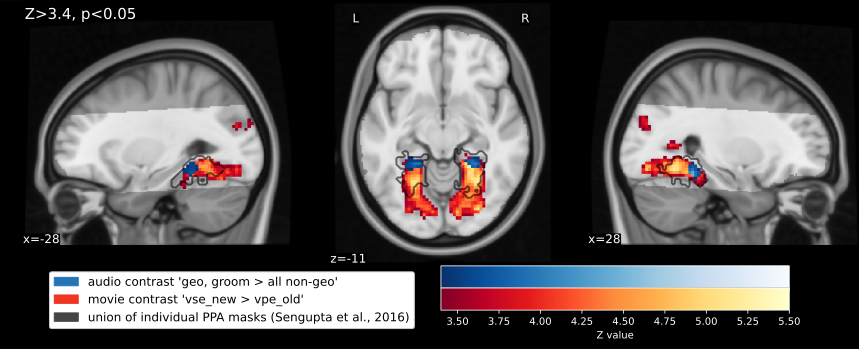
\includegraphics[width=\linewidth]{figures/group-slices}
    \caption{Mixed-effects group-level (N=14) GLM results. Significant clusters
        (Z>3.4, p<.05 cluster-corrected) are overlaid on the MNI152 T1-weighted
        head template (gray).
        Light gray: The audio-description's field-of-view
        (cf. \citep{hanke2014audiomovie}).
        Blue: the primary $t$-contrast for the audio-description comparing
        geometry-related nouns to non geometry-related nouns spoken by the
        audio-description's narrator (\texttt{geo, groom > all non-geo}).
        Red: the primary $t$-contrast for the movie comparing cuts to a new
        setting with cuts to a familiar perspective (\texttt{vse\_new >
        vpe\_old}).
        Black: outline of overlapping individual PPA ROIs      \citep{sengupta2016extension}.}
    \label{fig:group-slices}
\end{figure*}


\subsection{individual results}

\todo[inline]{other reasons than localization performance?}

% why individual results in the first place.
We also investigated localization performance of both naturalistic paradigms on
the level of individual subjects.
% results in both subject and group space
Time series of all subjects were analyzed both in group space and subject space.
% report here in group space
For better comparison of results across participants, we here report results
($z$-maps; Z>3.4, p<.05 cluster-corrected) of the analyses that was performed in
group space.
% ref to figure
Figure \ref{fig:subs-thresh-ppa} depicts thresholded $z$-maps of the primary AO
and AV $t$-contrast, and the outline of the individual PPAs
\citep{sengupta2016extension} overlayed on the MNI152 template (horizontal slice
z=-11 for all subjects).
% individual z-maps -> dataset
Results of the analyses that were performed in each subject's subject-space
(unthresholded $z$-maps and thresholded $z$-maps with Z>2.3, p<.05) can be found
in the accompanying dataset.
% results in detail voxels of significant clusters in PPA ROI (and  RSC
% liberally)
% sub-01 (m): PPA (l/r), AO (l/r), AV (-/r); RSC: AO (l/r), AV (-/-)
% sub-02 (m): PPA (l/r), AO (-/-), AV (-/r); RSC: AO (-/-), AV (-/-)
% sub-03 (f): PPA (l/r), AO (-/-), AV (-/r); RSC: AO (-/-), AV (-/-)
% sub-04 (f): PPA (-/r), AO (l/r), AV (-/r); RSC: AO (l/r), AV (-/-) !
% sub-05 (m): PPA (l/r), AO (-/-), AV (-/-); RSC: AO (-/-), AV (-/-)
% sub-06 (m): PPA (l/r), AO (l/r), AV (-/-); RSC: AO (l/-), AV (-/-)
% sub-09 (m): PPA (l/r), AO (l/-), AV (l/r); RSC: AO (l/r), AV (l/r)
% sub-14 (f): PPA (l/r), AO (l/r), AV (-/r); RSC: AO (l/r), AV (-/-)
% sub-15 (m): PPA (l/r), AO (l/r), AV (-/r); RSC: AO (l/r), AV (l/r)
% sub-16 (m): PPA (l/r), AO (l/r), AV (l/r); RSC: AO (l/r), AV (l/-)
% sub-17 (m): PPA (l/r), AO (l/r), AV (l/r); RSC: AO (l/r), AV (l/r)
% sub-18 (m): PPA (l/r), AO (l/r), AV (l/r); RSC: AO (l/r), AV (-/r)
% sub-19 (f): PPA (l/r), AO (l/r), AV (-/r); RSC: AO (l/r), AV (l/r)
% sub-20 (f): PPA (-/r), AO (-/-), AV (l/r); RSC: AO (-/-), AV (-/-)

% PPA ROI (Sengupta et al., 2016)
The dedicated localizer \citep{sengupta2016extension} shows ROIs in 12 of 14
subjects and unilateral right clusters in two subjects (sub-04, sub-20).
% subjective threshold
Individual ROIs were assessed by visually inspecting unthresholded $z$-maps, and
setting a subjectively best fitting $z$-threshold to isolate a ROI that matched
the PPA.
% AO
In the current analysis of the AO stimulus, we find significant bilateral
clusters in nine subjects, and one significant cluster in the left hemisphere of
sub-09.
% subj-04
In sub-04, two homologous clusters are apparent, whereas the dedicated localizer
yielded only one cluster in the right hemisphere.
% AV
For the AV stimulus, results show homologous clusters in five subjects, and
unilateral right clusters in seven subjects (of which one subjects yielded a
unilateral cluster in the dedicated localizer).
% difference to dedicated localizer
We find bilateral clusters in sub-20, whereas the dedicated localizer yielded
only one cluster in the right hemisphere.

\todo[inline]{concluding statements?}


\begin{figure*} \centering
    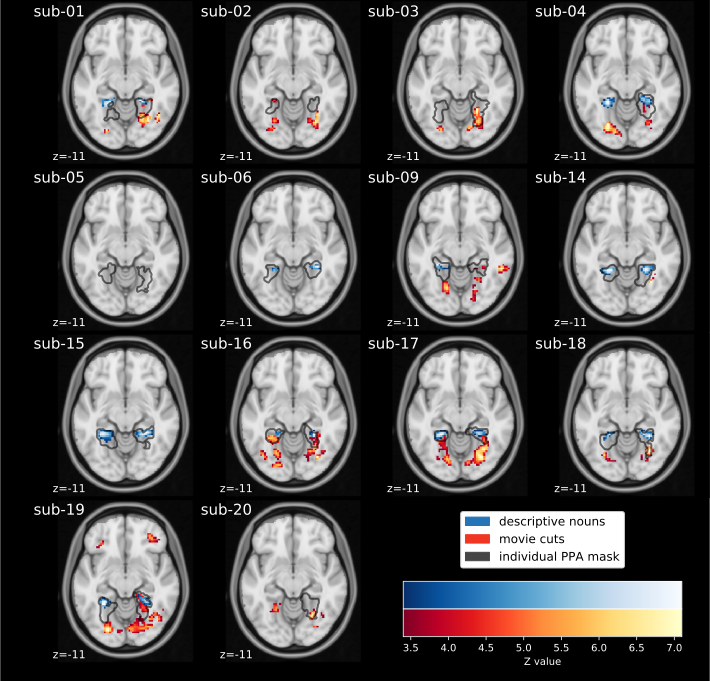
\includegraphics[width=\linewidth]{figures/subs-thresh-ppa}
    \caption{Fixed-effects individual-level GLM results (Z>3.4, p<.05
    cluster-corrected). To facilitate comparisons across subjects, individual
    brains are aligned via non-linear transformation to a study-specific T2*
    group template that is co-registered to the MNI152 template with an affine
    transformation (12 degrees of freedom).
    Light gray: The
    audio-description's field-of-view (cf.  \citep{hanke2014audiomovie}).
    Black: outline of the subject-specific PPA ROIs.
    Blue:
    the primary $t$-contrast for the audio-description comparing
    geometry-related nouns to non-geometry-related nouns spoken by the
    audio-description's narrator (\texttt{geo, groom > all non-geo}).
    Red: the
    primary $t$-contrast for the movie comparing cuts to an unfamiliar setting
    with cuts within an familiar perspective (\texttt{vse\_new > vpe\_old}).
    } \label{fig:subs-thresh-ppa} \end{figure*}


\subsection{Bland-Altman-Plots}

\todo[inline]{anything else to report here? seems more like just an explanation
of the plots}

% why it was done
To better depict the agreement (and difference) between individual results of
the dedicated visual localizer and contrast 1 of the AO paradigm, we created one
Bland-Altman-Plots for each of the 14 subjects (see Figure
\ref{fig:bland-altman}).
% x-axis
The x-axis of every subplot depicts the mean of $z$-values of two spatially
corresponding voxels taken from a subject's unthresholded $z$-map.
% y-axis
The y-axis of every subplot depicts the difference of $z$-values of two
spatially corresponding voxels (dedicated localizer minus AO stimulus).
% masking
We constrained the number of voxels in three ways as indicated by three colors
(grey, blue, red).
% masking in detail
Voxels were spatially constrained to a) voxels located in the occipital and
temporal lobes (gray; using the (probabilistic) Jülich Histological Atlas
\citep{eickhoff2005toolbox, eickhoff2007assignment}), b) voxels located in the
PPA overlap of all subjects (blue), and c) voxels located in the individual PPA
ROI(s)(red).
% top KDE plot
A shift of the distribution to voxels with a mean above zero can be seen the
further we constrain voxels to the individual PPA (see KDE plot for the x-axis).
% right KDE plot
Values above the horizontal line depict voxels that show a higher $z$-value in
the dedicated localizer, values below the horizontal line depict voxels that
show higher $z$-value in the AO stimulus.


\begin{figure*} \centering
    \includegraphics[width=\linewidth]{figures/subjs_bland-altman.png}
    \caption{Bland-Altman-Plots for individual subjects. The x-axis depicts the
        mean of two spatially corresponding voxels in the unthresholded z-map of
        the visual localizer and in the unthresholded z-map of contrast 1 of the
        AO stimulus (KDE plot on the top). The y-axis depicts the difference of
        two voxels (KDE plot on the right). The overlays depict voxels spatially
        contrained to be located in the temporal and occipital cortex (gray),
    PPA overlap of all subjects (blue), and individual PPA (red).}
    \label{fig:bland-altman} \end{figure*}


\subsection{stability contrasts}

\todo[inline]{I consider tables of significant clusters for every contrast as
overkill. Tables for just the ``primary contrast'', seems more appropriate; the
level of details explained depends on the discussion; atm moment I feel it
should be discussed more than expected; hence, following some notes as to dos}

\todo[inline]{as mentioned before: this section would also make sense to be at
the top or middle of the results; I moved it back and forth A LOT already}

\todo[inline]{s. comments for overview of sign. clusters in all contrasts}

% why we did different contrasts
We created different $t$-contrasts for the AO stimulus (see Table
\ref{tab:ao-contrasts}) and for the AV stimulus (see Table
\ref{tab:av-contrasts}) to test the stability of results across different
contrasts and exclude accidental findings.

% all AO contrasts
% 1 PPA (l/r); RSC (l/r), LOC (l/r)
% 2 PPA (l/r); RSC (l/r), LOC (l/r), r. sup.temp.C., r.fr.pole; putamen; etc
% 3 PPA (l/r); RSC (l/r), LOC (l/r),l&r sup.temp.C., anterior cing., paracing.
% 4 PPA (l/r); RSC (l/r), LOC (l/r)
% 5 PPA (l/r); RSC (l/r), LOC (-/-)
% 6 PPA (l/r); RSC (l/r), LOC (l/-), l&r sup.temp.C.; medial pref. c., precun
% 7 PPA (-/-); RSC (l/r), LOC (l/-), l&r sup.temp.C
% 8 PPA (-/-); RSC (-/-), LOC (-/-)
% control contrasts
% 9 PPA (-/-); RSC (-/r), LOC (-/-), left pars triangularis
%10 PPA (-/-); RSC (-/-), LOC (-/-)
%11 PPA (-/-); RSC (-/-), LOC (-/-),
%12 PPA (-/-); RSC (-/-), LOC (-/-), right posterior hippocampus
%13 PPA (-/-); RSC (-/-), LOC (-/-)

% results
The overlap of significant clusters of the eight contrast for the
audio-description, and five contrasts computed for the movie can be found in
Figure \ref{fig:stability-slices}.
% results in PPA
In the analysis of the AO stimulus, six of eight contrasts show significant
bilateral clusters in anterior regions of the group PPA
overlap.\todo[inline]{temporal occipital fusiform gyrus according to
Harvard-Oxford Cortical Structural Atlas}
% statement/answer
This suggest results are reproducible in a variety of contrasts and do not
depend on the design of one specific contrasts.
% individual results
Notably, we chose one contrast to look into individual results of all subjects
but individually a contrast different from the primary contrast might lead to
better individual localization results.\todo{concluding statements often feel
like interpretation/discussion to me}

% Precuneus = retrosplenial cortex ?
\todo[inline]{Seven of eight contrasts show bilaterally significant clusters in
the retrosplenial region (and ventral precuneus)}.

% transverse occipital sulcus
\todo[inline]{transverse occipital sulcus / occipital place area? in 6 of 8
contrasts (4 bilaterally)}

% confounds
\todo[inline]{``other clusters'' (confounds?): right superior temporal gyrus (4
contrasts); left superior temporal gyrus (3 contrasts); some prefrontal clusters
that show up in two contrasts}

% control in AO contrasts
\todo[inline]{control contrast essentially almost all none results; s. comments}

% all AV contrasts
% 1 PPA (l/r); RSC (l/r), LOC (l/r), VisC (l/r), intracalcarine, cuneal, ling.c
% 2 PPA (l/r); RSC (-/-), LOC (l/r), VisC (-/-)
% 3 PPA (l/r); RSC (-/-), LOC (-/-), VisC (-/r), occ. fusisf. g.
% 4 PPA (l/r); RSC (l/r), LOC (l/r), VisC (-/-), lingual g., occ. fusif. g.
% 5 PPA (l/r); RSC (l/r), LOC (l/r), VisC (-/-), occ. fusif. g.
% control contrasts
% 6 nothing
% 7 nothing
% 8 nothing
% 9 nothing
%10 se_new > se_old (nouns in AV stim): LOC (l/r)
% right PPA, bilateral sup. lat. occ. c., superior parietal lobe (right)

% AV intro
For the analysis of the AV stimulus, we created five contrasts for a cross-modal
comparison.
% PPA
All five AV contrasts yielded significant bilateral clusters in (temporal)
occipital, fusiform cortex showing congruency with the group overlap of
individual PPA ROIs.\todo{must be in posterior PPA as well}
% lingual gyrus
In three contrasts, these homologous clusters extend into the lingual
gyri.\todo[inline]{check regions and contrasts that are located outside of the
PPA; border of lingus belongs to PPA}
% RSC
Further, three contrasts show significant homologous clusters in the RSC.
% LOC
Lastly, four contrasts show significant homologous clusters in lateral occipital
cortices.
% statement/answer
Here again, we can show that results can in principle be accomplished by varying
the design of the contrasts.\todo{concluding statement =
interpretation/discussion?}

% control AV
\todo[inline]{control in AV stim: se\_new > se\_old (nouns in AV stim): LOC
(l/r), right PPA, bilateral sup. lat. occ. c., superior parietal lobe (right)}


\begin{figure*} \centering
    \includegraphics[width=\linewidth]{figures/stability-slices}
    \caption{Stability of contrasts. Overlap of significant clusters (Z>3.4;
        p<.05, cluster corrected) of contrasts created to isolate the PPA.
        Contrasts provide decreasing congruency with the spatial layout
        hypothesis and/or progressively less data/events. The overlap across
        contrasts is overlaid on the MNI152 T1-weighted head template (gray).
        Light gray: The audio-description's field-of-view (cf.
        \citep{hanke2014audiomovie}). Blue: contrasts 1-8 for the
        audio-description (see Table \ref{tab:ao-contrasts}. Red: contrasts 1-5
        for the audio-visual movie (see Table \ref{tab:av-contrasts}. Black:
        outline of overlapping individual PPA ROIs
        \citep{sengupta2016extension}.} \label{fig:stability-slices}
    \end{figure*}


\subsection{cross-modal and negative controls}

\todo[inline]{the contrasts are listed in the methods section. shall results of
these contrasts be reported here as well?}

\todo[inline]{there are only two control contrasts that yield significant
clusters. AO stimulus using annotation of movie cuts (vse\_new > pe\_old): right
RSC. AV stimulus using annotation of the narrator (se\_new > se\_old): right
PPA.}


\section{Discussion}

\todo[inline]{the biggest question: where does the discussion of the stability
of contrasts fit the best?}

\todo[inline]{in general: discussion explains how results fill gap identified in
intro}

\todo[inline]{provides caveats to the interpretation describes how paper
advances the field by providing new opportunities}

\todo[inline]{typically done by recapitulating the results, discussing
limitations, and then revealing how the central contribution may catalyze future
progress}

\todo[inline]{first paragraph summarizes the important findings from the results
section, focusing on their meaning}

% previous studies: visual
On the one hand, previous studies reported bilaterally increased hemodynamic
activity in the PPA when participants were watching static pictures of landscape
compared to face or objects (e.g. \citep{epstein1998ppa,
epstein1999parahippocampal})
% previous study: auditory
On the other hand, a study using spoken sentences reported mixed results
\citep{aziz2008modulation}.
% what we did
Hence, we use analogous statistical models in three different experimental
paradigms to compare results gained from a dedicated visual localizer to results
we gained from a movie and the movie's audio-description.
% We focus
Our results suggest that the perception of verbal spatial cues embedded in an
auditory narrative contrasted with non-spatial cues correlate with increased
activation in the PPA of both hemispheres.


\subsection{correlation of regressors}

\todo[inline]{could maybe pasted into method section to save space here; a short
interpretation is given there already}
% stimuli not designed for research purposes
Both naturalistic stimuli were not designed to be used in a BOLD fMRI experiment
but to entertain their audiences.
% why correlation matrix  was created
Thus, we first tested for correlation of regressors (s. \ref{fig:reg-corr}) that
are based on the annotated stimulus features because a high degree of shared
variance lowers detection power
% results of computing feature correlation
Results show no to minor correlations of regressors across all stimulus
segments.
% encouraged by that we build contrasts (statement)
Thus we felt encouraged to create traditional/canonical voxel-wise GLMs that
modeled and contrasted hemodynamic activity similarly to previous studies that
used simplified stimuli.


% The second through fourth paragraphs may deal with potential weaknesses
% linking it to the relevant literature or how future experiments can deal
% with these weaknesses.

% The fifth paragraph may then culminate in a description of how the paper moves
% the field forward.

% Discussion paragraphs often conclude by describing a clever, informal way of
% perceiving the contribution or by discussing future directions that can extend
% the contribution.

% step by step, the reader thus learns to put the paper’s conclusions into the
%right context.


\subsection{group level}

\todo[inline]{discuss only PPA here}
% intro
We performed whole-brain analyses on data from the audio-visual movie and its
audio-description. We chose one contrast of each stimulus to be investigated not
just on a group level but also on the level of individual subjects. Additional
contrasts were tested to investigate the stability of results across contrasts
when contrasted categories and the amount of available data is varied.


\subsubsection{AO stimulus}

% AO stimulus cluster location
Group results of the AO stimulus' primary contrast yielded spatially
concise / restricted clusters in the anterior part of the PPA group overlap
taken from \citep{sengupta2016extension}.
% diff to Aziz (2008)
Unlike \citep{aziz2008modulation} we did not use whole sentences as events to
model hemodynamic responses but modeled from on- to offset of single words
that cue the listener about the movie's missing visual content.
% conclusion
Our group results suggest that auditory spatial information does not just
modulate activity in the PPA (depending on other factors like familiarity; s.
\citep{aziz2008modulation}) but correlates with bilaterally increased
activation.\todo{``modulate'' suggests causation}

% transition to task topic
Moreover unlike most previous studies, our paradigm was free of any task.
%
Nevertheless, one early block-design study \citep{epstein1998ppa} compared
results from a paradigm that employed a (perceptual) judgment task of static
pictures to the same paradigm but without that task.
% results during no task
Hemodynamic activity was less but still significantly increased when
participants had no task to keep them alert and attentive to the stimuli.
% we have no task neither
Our paradigm is similar in that sense that our participants had no behavioral or
cognitive task (e.g. forming a mental image of the stimuli; cf.
\citep{ocraven2000mental})  but just had to ``enjoy the audio-description''.
% but we are still different
Our paradigm still differs from previous studies because the relevant stimulus
features were incidentally embedded in a continuous auditory stream.
% conclusion
This embeddedness prevents participants from making assumptions about the
investigated perceptual process by just being exposed to the paradigm and thus
mimics experiencing the world outside the lab more closely.
% concluding statement: kinda automatic process
The lack of a task further suggests verbal spatial information is processed in
the PPA in an automatic fashion and does not necessarily rely on deliberately
paying attention to spatial information.


\paragraph{shortcomings of AO contrasts}

\todo[inline]{cf. Methods: annotation \& Methods: AO copes}
% optimal stimulus type in vision
In the visual domain, landscapes and not pictures of landmarks or buildings are
considered to be the ``optimal'' stimulus type (cf. Epstein (1998, 1999, 2003,
2008).\todo{check references}
% cateogries in primary contrasts
In the current study's primary contrast, we compared verbal cues regarding
landmarks ((\texttt{geo}; often buildings or other single aspects of a whole
scene) and elements defining the geometry of a room/locale (\texttt{groom}) to
non-spatial cues.
% we did not choose se\_new and se\_old
Notably, we did not choose the categories that contained switches from one
setting to another (texttt{se\_new} and texttt{se\_old}) which one might assume
to contain the auditory equivalent to the ``optimal'' visual stimulus type.
% why not se\_new or se\_old
These categories were actually heterogeneous: they rarely contained whole (and
thus vague) descriptions of landscapes (e.g. ``in a football stadium'',
``Forrest is running through the jungle'') but mostly landmarks or buildings,
and also non-spatial cues.\todo{repeat examples from method section}.
% further studies
Given that humans can identify the gist of a rich visual scene within the
duration of a single fixation \citep{henderson2003human} further studies might
investigate if categories of wholistic but vague verbal descriptions of
landscapes correlate with differential hemodynamic activity in the PPA compared
to more concrete spatial cues.


\subsubsection{AV stimulus}
% location
Group results of the AV stimulus' primary contrast yielded bilateral clusters
that span the group overlap of individual PPAs from anterior to posterior and
expand into retrosplenial regions.
% difference in location/size to AO and VIS
Clusters also expand into more posterior regions (occipital fusiform gyrus,
lingual gyrus, and intracalcarine cortex)\todo{which of these regions overlap
with group ROI? which regions show clusters but do not overlap with PPA?}
% confound of higher perception
This can be attributed to the fact that we averaged the content of individual
frames after a cut and did not control for confounding features like depicted
faces or objects.
% confounds of lower perception
It further suggest low-level visual features were not averaged out leading to
clusters spanning the intracalcarine cortex.
% further studies
Since the capability to isolate clusters or networks correlating with specific
perceptual (or cognitive) processes is influenced by the amount of annotated
stimulus features further studies focusing on visual perception should annotate
and model visual features of naturalistic stimuli more rigorously.\todo{ouf,
okay...}
% cross-modal control purpose?
\todo[inline]{concluding statement regarding AV vs AO and cross-modality of
results?}


\subsection{stability of contrasts}

\todo[inline]{the pain starts exactly here}

% why we did a couple of contrasts
For both stimuli we created additional contrasts that varied the amount of
events available for the analysis and how well the annotated events within
categories on average matched the stimulus type that we assumed to be
preferentially processed in the PPA.

\subsubsection{PPA}
% PPA AO
Regarding contrasts of the AO stimulus, six of eight contrasts show
significant bilateral clusters in the anterior part of the group PPA.
% PPA AV
Regarding contrasts of the AV stimulus, all five contrasts show significant
bilateral clusters in the PPA but extending into posterior regions
% no incidental findings
Results of the additional contrasts suggest that bilaterally increased
activation in the PPA does not depend on accidental findings but is are stable
across contrasts of the movie and the audio-description.

% but
Results also suggest that localization performance depends on the
amount of available data and how well the feature space is modeled.
% what's going on
Despite performing a whole brain analysis, we do not find many (random) clusters
in single contrasts or even systematically across contrasts that hamper the
interpretation of results.\todo[inline]{god forgive me for this paragraph}.
% null results regarding attention and eye movements
For example in the AV results, we do not find significant clusters that could be
attributed to cognitive processes like attention, eye movements, or
memory.\todo{which kind of memory}

% BUT: amount of data
Nevertheless, localization performance is influenced by the amount of available
data\todo{give examples of contrast using less events in AV and AO} and how well
events within categories matched on average the preferred stimulus type.
% example AV: data amount and category homogeneity
For example in the AV stimulus, we averaged different kind of movie cuts
regardless to the movie frames content.\todo[inline]{how well spatially
constrained are the clusters?}
% results
As a result, clusters are more widespread and reach into early visual cortex.

\todo[inline]{first: number of available events -> ``noise''}

\todo[inline]{second: category match -> ``localization performance''}

% AO: stimulus categories
For example in the AO stimulus, nouns of the narrator that cue a switch to
another setting belong to different categories (s. above).\todo[inline]{Number
of events in which contrasts?}
% example for data amount AO: superior temporal cortex
In four of nine contrasts of the AO stimulus, we find significant clusters in
superior auditory cortices (including early auditory cortices?)\todo{which
exactly}
% conclusion
This suggests that variance correlating with lower level auditory processes was
(not) averaged (out) across trials\todo{which contrasts; A1 \& low-level
nuisance regressors?}
% foreshadowing of narrator by soundscape
Further, verbal cues are regularly forestalled by changes of the
soundscape.\todo{cross-modal control contrasts; all negative results at moment
of cuts but vse\_new > pe\_old): right RSC.}
% arnott
\todo[inline]{e.g. arnott2008crinkling find increased activations of PPA to
sound made by objects}
% hypothesis
We hypothesize that not just semantic information but also the mere changes of a
soundscape that cues a listener about a setting's spatial layout of could
correlate with increased activity in the PPA.
% conclusion: AO and AV stability
In summary, our results across add further evidence that model-driven analyses
can be run on data from naturalistic stimuli to isolate brain activity
correlating with specific perceptual processes.
% but
Nevertheless isolation performance relies on how well the model captures
different aspects of the stimuli's feature space.


\subsubsection{other systematics: anterior vs. posterior, RSC and OPA}

% intro
Nevertheless, results across contrasts of both stimuli show significant clusters
constrained to the anterior part of the PPA in contrasts of the AO stimulus, and
significant clusters in the retrosplenial cortices and superior lateral cortices
in both naturalistic stimuli.

\subsection{anterior vs posterior PPA: contextual associations}

\todo[inline]{at the moment it makes more sense to discuss it sooner; but it
kinda depends on stuff that is happening in the RSA too}

% Aminoff (2013)
Aminoff (2013) in general: processing of strong,
long-term, contextual associations elicits activity within the PHC, as well as
the RSC (which includes regions of the retrosplenial cortex, extending into the
posterior cingulate cortex, and the precuneus), the medial prefrontal cortex
(MPFC), and the transverse occipital sulcus (TOS) (Figure 2) [2,3,59–67].

% contextual associations in anterior vs. posterior
Aminoff et al. (2013): We propose that the general function of the PHC can be
thought of as processing of contextual associations. A subregion of the
posterior PHC is particularly optimized to process spatially organized
contextual associations, whereas more anterior regions of the PHC are optimized
to process contextual associations in other, non-spatial domains.
% posterior PPA for visual visual associative information
Spatial contextual associations are a dominant property of places and scenes,
and thus scenes consistently activate this posterior subregion of the PHC (e.g.,
PPA; Epstein, 1998). We do not argue that the PHC is not sensitive to
spaces, places, and spatial information, but rather that it is sensitive to
spatial stimuli because of the associative information (space-related
associations) that such stimuli evoke.

% Aminoff regarding contextual processing in the PHC and beyond
Aminoff et al. (2013). We compared contextual processing of
objects that are strongly related to a specific place (e.g., an oven is found in
a kitchen) with contextual processing of objects that are highly associated with
a context but not a specific place (e.g., a birthday cake is found at a birthday
party, but the party can take place anywhere, at home, in a restaurant, at a
park). Activity elicited by these two types of contextual objects was compared
with the activity elicited for objects that were only weakly associated with
many contexts (e.g., a lamp). Differential activity was found in the PHC and the
RSC, replicating the previous findings (Bar \& Aminoff, 2003, The
parahippocampal\dots).
% results
Activity within the PHC, however, was distributed along
an anterior–posterior axis, with activity related to spatial contexts focused in
the posterior part of the PHC and activity evoked by non-spatial contexts
focused in the more anterior part of the PHC (Bar \& Aminoff, 2003, Cortical
analysis of visual context; Aminoff et al., 2007, The parahippocampal cortex
mediates spatial and nonspatial associations).

\subsection{anterior vs posterior PPA}
% connectivity
Aminoff et al. (2013) regarding Baldassano (2013): some evidence from a human
neuroimaging study examining functional connectivity of differences between
anterior and posterior regions of the PHC show that the anterior regions are
more functionally connected to retrosplenial complex (RSC) and parietal
cortices, whereas the posterior regions are more functionally connected to
visual processing regions.

% Baldassano (2013). Differential connectivity with Parahippocampal Place Area
Baldassano (2013). We utilize a functional connectivity measure for fMRI that
can estimate connectivity differences at the voxel level. We provide the first
direct evidence that anterior and posterior PPA exhibit distinct connectivity
patterns. Anterior PPA is more strongly connected to regions in the default mode
network (including the parieto-medial temporal pathway). Posterior PPA more
strongly connected to occipital visual regions.
% gradient
We show that object sensitivity in PPA also has an anterior–posterior gradient,
with stronger responses to abstract objects in posterior PPA.
% summary
Our results (and previous work) suggest that posterior PPA is concerned
primarily with perception of low-level visual features and object shape, while
anterior PPA is involved in memory and global contextual processing.

% from Baldassano discussion
Our results demonstrate that PPA exhibits a gradient in connectivity along
anterior–posterior axis (analogous to the gradient in connectivity along macaque
TH/TF/TFO). The connectivity gradient was also paired with a functional gradient
of sensitivity to scene and abstract object stimuli. These results demonstrate
that anterior and posterior PPA connect differentially to two distinct cortical
networks.
% but not independent
Our data suggest that PPA might contain identifiable subregions, but subregions
should not be considered as completely independent modules. Both subregions
activate selectively to scenes, and the parahippocampal region (at least in
macaques) is densely self-connected (Suzuki, 2009), implying that these
subregions cooperate to build a complete representation of a scene.  Their
distinct connectivity properties, however, suggests that each may be involved in
specific aspects of visual and cognitive processing involved in the overarching
goal of scene understanding.
% posterior PPA
Posterior PPA shows a stronger response to abstract objects than anterior PPA,
and is more strongly connected to all of occipital visual cortex, including LOC
and TOS. These regions have well-defined retinotopic maps (Arcaro et al., 2009;
Nasr et al., 2011), and are associated with the perception of low-level visual
features and object shape. Previous work has hinted that posterior PPA is more
responsive to both simple visual textures and objects; Arcaro et al. (2009)
found that a posterior portion of PPA responded about four times as strongly to
a flickering checker-board stimulus compared to an anterior portion, and that
the response to objects was greater than the response to scrambled images only
in the posterior portion => posterior PPA may be more visually responsive than
anterior PPA.
% LLA
Our description of posterior PPA is in fact similar to the original proposal of
Aguirre et al. for a “lingual landmark area” (LLA), slightly posterior to PPA,
which was “specialized for the perception of visual stimuli with orienting
value” (Aguirre et al., 1998) and carried out bottom-up perceptual analysis to
recognize locations or landmarks (Cant and Goodale, 2007; Epstein et al., 1999).
Although the LLA is no longer identified as an independent region from PPA in
current studies, it is possible that the posterior portion of PPA corresponds to
the properties of the proposed LLA, offering an explanation for why this region
was localized more posteriorly than the full PPA.
% Anterior PPA
Anterior PPA is specifically connected to RSC, cIPL, medial PFC, and the lateral
surface of the anterior temporal lobe. In addition, this portion of PPA is less
visually responsive to both scenes and objects, with notably low sensitivity to
abstract object stimuli.

% DMN
The set of regions connected more strongly to anterior PPA is strikingly similar
to the Default Mode Network (DMN) (Buckner et al., 2008; Fox et al., 2005;
Raichle et al., 2001), which is known to include the parahippocampal region. The
only portions of the DMN that do not show differential connectivity to anterior
PPA in our data are the rostral portion of the posterior cingulate cortex (PCC)
and the superior frontal cortex.
% PPA and DMN
DMN has been implicated in a large number of internally-focused
tasks, one of its key roles involves autobiographical memory (Buckner et al.,
2008). Models of recognition memory have previously identified parahippocampal
cortex as primarily encoding spatial context information (Eichenbaum et al.,
2007). Data from Aminoff et al. (2007) has suggested that an anterior
portion of PPA may be involved in recall based on spatial context. Our results
are consistent with anterior PPA playing a more central role in memory than
posterior PPA, given anterior PPA's connectivity with the DMN.
%
The fact that anterior PPA had a lower sensitivity to our abstract object
stimuli does not necessarily imply that this region does not use object
information. Previous work has shown that PPA responds to objects that have
spatial associations (Aminoff et al., 2007), are space-defining (Mullally and
Maguire, 2011), and are navigationally-relevant (Janzen and Van Turennout,
2004). These types of responses require spatial memory and cannot be based
purely on visual features like object shape. If anterior PPA is involved in
processing spatial context, then space-defining or navigationally-relevant
objects could activate anterior PPA more strongly than our abstract objects,
which were unfamiliar and provided no sense of context or orientation. Further
experiments will be required to determine what type of object-related
information is used in this region.



\paragraph{RSC (in both stimuli)}

\todo[inline]{check location in primary contrast and in overlap of contrasts}

% but RSC
Apart from the PPA, we find significantly increased activity consistently across
contrast of both contrasts in the retrosplenial cortex (RSC).\todo{how many
exactly?}

% location functionally defined
In context of a scene-responsive region, the RSC is functionally defined and not
necessarily identical to the anatomically defined retrosplenial cortex [26]
\citep{epstein2008parahippocampal}.
% location
The RSC is located in the retrosplenial cortex, and posterior cingulate region,
near to the point where the calcarine sulcus joins the parietal-occipital sulcus
\citep{epstein2008parahippocampal}.
% anatomy of real RSC
The Retrosplenial cortex (BA 29 and 30) adjoins and is partially encircled by
the posterior cingulate (BA 23 and 31) [51–56]
\citep{epstein2008parahippocampal}.
% function
RSC is strongly active during scene viewing, scene imagery [25] and mental
imagination of navigation through familiar environments [8]
\citep{epstein2008parahippocampal}.
% conclusion
\todo[inline]{interpretation?; cf.\citep{vann2009what}}

\todo[inline]{conclusion?}

\paragraph{superior lateral occipital cortex (in both stimuli)}

\todo[inline]{e.g. Dilks, Kanwisher (2013). The Occipital Place Area Is Causally
and Selectively Involved in Scene Perception?}



\subsection{negative controls and cross-modal controls}

\todo[inline]{could be mentioned in a few sentences. But above topics a far too
much still; better embed somewhere above}


\subsection{individual analyses}

\todo{how to discuss Bland-Altman-Plots? Please, let's talk about that shortly}

\todo{discussion of individual differences? what do the results suggest???}


\subsubsection{AO stimulus}

\todo[inline]{shortcoming: no task to attend to spatial information}

\todo[inline]{different level of alertness during paradigms}

\todo[inline]{individual ``preference'' to pay attention to
spatial infos (which contradicts statement above that attention is not a
prerequisite)}

\todo[inline]{different ``capability'' to process auditory spatial information}

% intro
We checked the results of the primary contrast also on the level of individual
subjects to ``test'' the audio-description's performance as a functional
localizer compared to the dedicated visual localizer paradigm.\todo{hm, sounds
meh}
% results of dedicated localizer
The dedicated localizer \citep{sengupta2016extension} yielded bilateral ROIs in
12 of 14 subjects and unilateral right ROI in two subjects (sub-04, sub-20).
% in the current study
The audio-description's primary contrast yielded significant bilateral clusters
in 9 of 14 subjects (of which sub-04 shows just right-lateralized PPA ROI)  and
an unilateral significant cluster in one subject.
% difference
Notably, we here used a ``one fits all approach`` whereas
\citep{sengupta2016extension} chose the best fitting $z$-threshold in a
subject's unthresholded $z$-maps by visual judgment and used the best of three
alternative contrasts (strict, relaxed, or simple contrast).
% quote from Hanke (2014)
Hanke et al. (2014): Compared to AV stimulus, the AO stimulus leaves a much
larger margin for inter-individual differences in imagining scenery, as well as
actors' character and personality traits, while still preserving the time-locked
presentation of information to a listener. At the same time, the AO stimulus
limits the effect of an attentional focus on the selection of a subset of
simultaneously occurring auditory events, in contrast to the selection of
different parts of the visual field.
% conclusion
Our results suggest that a naturalistic auditory stimulus is suitable to
localize (the anterior part) of a higher-level visual area in the majority of
subjects.
% individual contrasts
Nevertheless, studies that primary aim for individual results should
choose individual thresholds and test more than just one contrast to gain the
best (?) individual ROIs.\todo{``best'' always sounds kind of judgmental}


\subsubsection{AV stimulus}
% intro
On individual level, mixed results for AV stimulus.
\todo{give the numbers}

\todo[inline]{which contrast works better in which subjects?; if focus is
individual diagnostics take the individually best contrasts; cf. Sengupta}

% shortcomings
visual confounds all over the place; obvious solution: annotate frames and track
focus of attention (but gist of a frame vs. attentional focus)

Individual differences when seeing a whole picture with many features vs. serial
auditory stream of information providing incidental cues; spatial attention?






\section{Conclusions}

\todo[inline]{template has no section ``conclusion'' -> use the last paragraph}

% natural stimulation
Intro: Natural stimuli like movies \citep{hasson2008neurocinematics,
sonkusare2019naturalistic} or narratives \citep{honey2012not,
lerner2011topographic, silbert2014coupled} offer an easy to implement,
(continuous,) complex, immersive, task-free paradigm that more closely resembles
our natural dynamic environment than traditional experimental designs.
% why naturalisti stimuli are so cool
(see also \citep{sonkusare2019naturalistic, eickhoff2020towards,
hamilton2018revolution})
% re-use of data for independent research question
Due to their continuity, complexity, and length, they offer a vast amount of
data on a variety of brain functions like low-level perception, attention,
comprehension, memory, emotions, or social interactions. This suggests the data
can later be reused for variety of totally different, independent research
questions, possibly on an individual level; increased compliance in individual
diagnostics in ``special'' populations where compliance is more difficult to
archive (pediatric or psychiatric)

% we annotated a couple of features to build contrasts
Method: The feature ``auditory spatial information'' is just one example of a
stimulus feature that can be annotated and used to build a model.
% data-driven vs. model-driven
Why we used a traditional GLM...

% results
Results: Our results demonstrate...

% conclusion auditory localizer
Conclusion: Thus, a complex but naturally engaging auditory stimulus like an
audiobook might in principle be used as a non-visual localizer for a variety of
brain functions in subjects who are not willing or able to follow task
instructions during brain scanning.


\subsection*{Code availability}
% wo kommt dieser Abschnitt hin?  how to write Code availability statement
% https://www.springernature.com/gp/authors/research-data-policy/data-availability-statements/12330880
\todo[inline]{provide supporting source code, and explaining how and where
others may access all data underlying the analysis} \emph{for all studies using
    custom code in the generation or processing of datasets, a statement must be
    included here, indicating whether and how the code can be accessed,
including any restrictions to access; include information on the versions of any
software used, if relevant, and any specific variables or parameters used to
generate, test, or process the current dataset. }

\section*{Acknowledgements}
% Text acknowledging non-author contributors. Acknowledgements should be brief, and should not include thanks to anonymous referees and editors, or effusive comments. Grant or contribution numbers may be acknowledged.
% Author contributions Please describe briefly the contributions of each author to this work on a separate line.
\emph{COH did this and that.
MH did this and that.
We are grateful to \href{www.florianschurz.de}{Florian Schurz} who initiated doing the annotation of the descriptive nouns, and performed the preliminary annotation of nouns.}

\section*{Competing financial interests}
\emph{A competing financial interests statement is required for all accepted
papers published in \emph{Scientific Data}. If none exist simply write,
``The author(s) declare no competing financial interests''.}

\section*{Figures Legends}
\emph{Figure should be referred to using a consistent numbering scheme through
the entire Data Descriptor. For initial submissions, authors may choose
to supply this document as a single PDF with embedded figures, but
separate figure image files must be provided for revisions and accepted
manuscripts. In most cases, a Data Descriptor should not contain more
than three figures, but more may be allowed when needed. We discourage
the inclusion of figures in the Supplementary Information \textendash{}
all key figures should be included here in the main Figure section.}

\emph{Figure legends begin with a brief title sentence for the whole figure
and continue with a short description of what is shown in each panel,
as well as explaining any symbols used. Legend must total no more
than 350 words, and may contain literature references.}

\section*{Tables}

\emph{Tables supporting the Data Descriptor. These can provide summary information
(sample numbers, demographics, etc.), but they should generally not
be used to present primary data (i.e. measurements). Tables containing
primary data should be submitted to an appropriate data repository.}

\emph{Tables may be provided within the \LaTeX{} document or as separate
files (tab-delimited text or Excel files). Legends, where needed,
should be included here. Generally, a Data Descriptor should have
fewer than ten Tables, but more may be allowed when needed. Tables
may be of any size, but only Tables which fit onto a single printed
page will be included in the PDF version of the article (up to a maximum
of three).}

{\small\bibliographystyle{unsrtnat}
\bibliography{references}}

%\begin{thebibliography}{1}
%\expandafter\ifx\csname url\endcsname\relax
%  \def\url#1{\texttt{#1}}\fi
%\expandafter\ifx\csname urlprefix\endcsname\relax\def\urlprefix{URL }\fi
%\providecommand{\bibinfo}[2]{#2}
%\providecommand{\eprint}[2][]{\url{#2}}
%
%\bibitem{cite1}
%\bibinfo{author}{Califano, A.}, \bibinfo{author}{Butte, A.~J.},
%  \bibinfo{author}{Friend, S.}, \bibinfo{author}{Ideker, T.} \&
%  \bibinfo{author}{Schadt, E.}
%\newblock \bibinfo{title}{{Leveraging models of cell regulation and GWAS data
%  in integrative network-based association studies}}.
%\newblock \emph{\bibinfo{journal}{Nature Genetics}}
%  \textbf{\bibinfo{volume}{44}}, \bibinfo{pages}{841--847}
%  (\bibinfo{year}{2012}).
%
%\bibitem{cite2}
%\bibinfo{author}{Wang, R.} \emph{et~al.}
%\newblock \bibinfo{title}{{PRIDE Inspector: a tool to visualize and validate MS
%  proteomics data.}}
%\newblock \emph{\bibinfo{journal}{Nature Biotechnology}}
%  \textbf{\bibinfo{volume}{30}}, \bibinfo{pages}{135--137}
%  (\bibinfo{year}{2012}).
%\end{thebibliography}

\section*{Data Citations}

Bibliographic information for the data records described in the manuscript.

1. Lastname1, Initial1., Lastname2, Initial2., ...\& LastnameN, InitialN. \emph{Repository name} Dataset accession number or DOI (YYYY).

\end{document}
\documentclass[english]{article}
